% !TeX root = ../libro.tex
% !TeX encoding = utf8

\setchapterpreamble[c][0.75\linewidth]{%
	\sffamily
  \emph{Hemos perfeccionado el ordenador de propósito general para cálculos científicos. Ahora intentamos emplear el mismo dispositivo con pequeñas modificaciones en una gran variedad de situaciones diferentes para las cuales no fue diseñado en primer lugar. En estas circunstancias, si llegara a resultar que la lógica básica de una máquina diseñada para la solución numérica de ecuaciones diferenciales coincide con la lógica básica de una máquina destinada a hacer facturas para una tienda departamental, consideraría esto como la coincidencia más asombrosa que haya encontrado.}
 \begin{flushright} — Howard Aiken, \cite{Aiken1956} \end{flushright}
% \\[8pt]
	\par\bigskip
}
%\vspace{28pt}

\chapter{Programas en Python y máquinas de Turing}\label{ch:programas-python-maquinas-turing}

La máquina de Turing, inventada por Alan Turing en 1937 \cite{Turing1937}, es un modelo matemático sencillo que pretende representar la noción de algoritmo, y del que hablaremos en detalle en la \cref{sec:maquinas-turing}. Esta máquina es una de las herramientas más relevantes en las ciencias de la computación, pues su simplicidad permite resolver potentes resultados, como la no decibilidad del problema de parada (\cref{prop:parada-no-decidible}), a partir del cual podremos adentrarnos en la cuestión principal de nuestro trabajo: la incompletitud de las matemáticas. Sin embargo, esta potencia formal tiene una desventaja, que comprobaremos a partir de un simple ejemplo (\cref{ej:mt-1}): definir programas sencillos en este modelo es complejo y tedioso.

Este inconveniente es el que motiva este capítulo: en la \cref{sec:equivalencia} probaremos la equivalencia entre los programas de ordenador (en nuestro caso, los programas en Python, que exploraremos en la \cref{sec:programas-python}) y las máquinas de Turing. Esto nos permitirá ver un programa en Python como una representación de una máquina de Turing, eliminando el principal inconveniente y quedándonos con la potencia matemática ya comentada.

Es importante resaltar que los resultados que aquí aparecen son perfectamente generalizables a cualquier lenguaje de programación. Sin embargo, decidimos usar este lenguaje por su facilidad de comprensión y de uso.

Tanto el resultado de equivalencia que probamos en este capítulo como la observación anterior son especialmente interesantes, ya que guardan una fuerte relación con la tesis de Church-Turing, de la que hablaremos brevemente en la \cref{sec:church-turing}.

\section{Programas en Python}\label{sec:programas-python}

%% Introducción al lenguaje de programación

Python\index{Python} \cite{Martelli2006} es un lenguaje de programación de alto nivel, interpretado, orientado a objetos y \emph{open source}, ampliamente usado en la actualidad para una gran variedad de aplicaciones. Una de sus principales características es su legibilidad y facilidad de uso: cualquier persona experimentada en otros lenguajes podrá comprender y redactar programas en Python con mucha sencillez.

Usando Python, podemos escribir una gran variedad de programas. Para el propósito de nuestro estudio, nos centraremos en una clase de programas específica: aquella que tiene únicamente una cadena de caracteres (\emph{string}) como entrada y una cadena de caracteres como salida. Los llamaremos \emph{programas SISO} (del inglés, \emph{Single Input-Single Output}, ver \cref{def:programa-siso}). \cite{MacCormick2018} En breve, comprobaremos cómo esta clase no es restrictiva: estos tipos de programas son tan expresivos como cualquier otro programa. De hecho, en este trabajo, usaremos los términos ``programa'' y ``programa SISO'' indistintamente, y en ambas ocasiones nos referiremos a un programa en Python de tipo SISO.

% ====================
\begin{definicion}[Función SISO]\label{def:funcion-siso}
\index{función!SISO}
Definimos una \emph{función SISO} como una función de Python que acepta un único parámetro de tipo \emph{string} como entrada, y que devuelve un \emph{string}.
\end{definicion}
% ====================

% ====================
\begin{definicion}[Programa en Python de tipo SISO]\label{def:programa-siso}
\index{programa SISO}
Respecto a un sistema informático de referencia $C$, definimos un \emph{programa en Python de tipo SISO} como una cadena de caracteres $P$, de modo que:

\begin{itemize}
    \item $P$ es código en Python sintácticamente correcto;
    \item $P$ define al menos una función, y la primera de ellas es de \emph{tipo SISO}. A esta función la llamaremos \emph{función main}.
\end{itemize}
\end{definicion}
% ====================

Observemos que en la definición anterior se especifica un sistema informático $C$,\index{sistema informático} pero no se define de forma explícita. Podemos pensar en $C$ como cualquier sistema informático, con cualquier configuración de \emph{software} y \emph{hardware}, y con tanta memoria como sea necesaria.

También podemos preguntarnos por qué queremos decir cuando nos referimos a un programa ``sintácticamente correcto'', dado que esto dependerá de varios factores, como la versión de Python instalada en $C$, así como el sistema operativo, arquitectura, etc. Es posible que un programa se ejecute en un sistema $C$ y falle o incluso de una salida diferente en otro sistema $C'$. Sin embargo, y como veremos más adelante, usaremos estos programas como representaciones de máquinas de Turing. Los programas que presentamos aquí son independientes de arquitectura y de memoria, y las demostraciones que figuran en este trabajo son independientes de todas estas características.

También necesitaremos definir cuál es la salida de un programa en Python.

% ====================
\begin{definicion}[Salida de un programa]\label{def:salida-programa}
\index{salida!de un programa}
Sea $P$ un programa en Python respecto a un sistema informático $C$. Sea $M$ la función \emph{main} de $P$, e $I$ la \emph{entrada} de $P$, una cadena de caracteres. La \emph{salida de $P$ respecto a la entrada $I$}, $P(I)$, se produce usando $C$ para ejecutar $P$ con entrada $I$, y se define como:

\begin{itemize}
    \item Si $M$ devuelve una cadena de caracteres $O$, entonces $P(I)=O$.
    \item Si $M$ devuelve cualquier otro objeto en Python, entonces $P(I)$ no está definido.
    \item Si $M$ lanza una excepción,\footnote{Nos referimos a las excepciones que se pueden definir implícitamente en el lenguaje o que pueden resultar de errores en su uso, dado que en la definición de $P$ el programa es correcto sintácticamente.} entonces $P(I)$ no está definido.
    \item Si $M$ no termina, entonces $P(I)$ no está definido.
\end{itemize}

\emph{Nota.} La definición anterior puede ser generalizada fácilmente para $n$ entradas. Reemplazando $I$ por $I_1, I_2, ..., I_n$ obtenemos la definición correspondiente para $P(I_1, I_2, ..., I_n)$.
\end{definicion}
% ====================

% ====================
%\begin{nota*}\label{nota:multiples-parametros}

%NOT USED

%Para ello, basta definir las funciones $MAU$ y $UAM$.

%En primer lugar, la función $MAU$ (de ``{Múltiple A Uno}''), tiene como entrada $n$ cadenas de caracteres, $I_1, I_2, ..., I_n$, y produce como salida una única cadena de caracteres que surge de unir las cadenas $I_i$ mediante un separador \texttt{SEP}, que es también una cadena de caracteres. Usando $+$ como operador de concatenación, tenemos que:
%$$
%    MAU(I_1, I_2, ..., I_n; \texttt{SEP}) = I_1 + \sum_{i=2}^{n}\left(\texttt{SEP} + I_i\right) = I_1 + \texttt{SEP} + I_2 + \texttt{SEP} + ... + \texttt{SEP} + I_n
%$$
%Es importante que el separador \texttt{SEP} no se encuentre en ninguna de las entradas $I_i$, para que la ejecución de la función \texttt{UAM} no de lugar a ambigüedad.

%Definimos $UAM$ (de ``{Uno A Múltiple}''), que tiene como entrada una cadena de caracteres $I$ y un separador \texttt{SEP}, y como salida las cadenas de caracteres que surgen de separar $I$ usando el separador \texttt{SEP} como delimitador.

%Las funciones $MAU$ y $UAM$ están implementadas en la librería \texttt{utilidades}.

%Supongamos que tenemos una función \texttt{multiple} con $n$ entradas. Entonces, podemos convertirla en una función \emph{main}, \texttt{multiple\_main}quisiésemos implementar una función \texttt{multiple}, con múltiples entradas, basta definir:

%\begin{lstlisting}[language=Python, caption=\lstinline{una_a_múltiples_entradas.py},label={lst:una-a-múltiples-entradas}]
%import utilidades

%def multiple(entrada):
%    multiples_entradas = utilidades.UAM(entrada)
%    return funcion_multiple(*entrada)

%def funcion_multiple(entrada_1, entrada_2, ..., entrada_n):
%    # cualquier función
%\end{lstlisting}

%Y podremos llamar la función con
%WIP hacerlo con \texttt{mult\_a\_uno} y \texttt{uno\_a\_mult}
%$$
%    I_1 + \sum_{i=2}^{n}\left(\texttt{SEP} + I_i\right) = I_1 + \texttt{SEP} + I_2 + \texttt{SEP} + ... + \texttt{SEP} + I_n
%$$

%\begin{lstlisting}[language=Python, caption=\lstinline{una_a_múltiples_entradas.py},label={lst:una-a-múltiples-entradas}]
%def una_a_múltiples_entradas(una_entrada):
%    múltiples_entradas = una_entrada.split(SPLIT_CHAR)
%    return funcion_múltiples_entradas(*múltiples_entradas)

%def funcion_múltiples_entradas(entrada_1, entrada_2, ..., entrada_n):
%    # cualquier función
%\end{lstlisting}
%\end{nota*}
% ====================

En otras palabras, la salida de un programa es la cadena de caracteres devuelta por su función \emph{main} en caso de que lo haga, y no estará definida en caso contrario.

Al definir los programas en Python que usaremos en este trabajo, nos centramos en el uso de cadenas de caracteres (también llamadas \emph{strings})\index{string} como entrada y salida, y evitamos el uso de otros objetos de Python que no sean \emph{strings}. Inicialmente, podemos pensar que esto impone una limitación sobre los programas en Python que podemos escribir, pero esto realmente no es así. Para ello, basta observar que que cualquier objeto en Python puede ser codificado debidamente mediante una cadena de caracteres. Existen liberías nativas que permiten hacer esto, como \lstinline{pickle}.\footnote{La librería \lstinline{pickle} puede codificar y descodificar una gran variedad de tipos de datos, incluyendo todos los nativos. Tiene algunas limitaciones para objetos más complejos pero, dado que todos los objetos se pueden reducir estos tipos de datos, podemos afirmar que cualquier objeto puede ser codificado. \cite{Lutz2013}} Un ejemplo de esto se muestra en el \cref{lst:funcion-con-objeto-codificado}. La función \texttt{funcion\_con\_objeto\_codificado} es una función \emph{main}.
\vspace{8pt}
% ====================
\begin{lstlisting}[language=Python, caption=\lstinline{funcion_con_objeto_codificado.py},label={lst:funcion-con-objeto-codificado}]
import pickle

def funcion_con_objeto_codificado(codificado):
    descodificado = pickle.loads(codificado)
    # realizamos las operaciones que queramos con el objeto descodificado
    # el objeto descodificado puede ser de cualquier tipo

# creamos un objeto, por ejemplo, una matriz
adyacencias = {1:2, 3:4, 5:3, 4:2}

# serializamos (codificamos) el objeto a un string
adyacencias_codificado = pickle.dumps(adyacencias)

# podemos ahora ejecutar este objeto dentro de una función SISO
funcion_con_objeto_codificado(adyacencias_codificado)
\end{lstlisting}
% ====================

En la línea 1 importamos la librería \texttt{pickle}, que incorpora dos funciones:
\begin{itemize}
    \item \texttt{dumps} convierte un objeto cualquiera a una cadena de caracteres. En la línea 12, serializamos el objeto \texttt{adyacencias} a un \emph{string}.
    \item \texttt{loads} convierte la cadena de caracteres al objeto correspondiente. En la línea 4, ``descodificamos'' la cadena de caracteres, obteniendo en este caso el objeto \texttt{adyacencias}.
\end{itemize}
En resumen, hemos visto cómo la condición de ser SISO para un programa en Python no es realmente una restricción. \label{lab:siso-no-restr} Sin embargo, esta clase de problemas nos resultará muy conveniente, como veremos más adelante.

% ====================


\section{Máquinas de Turing}\label{sec:maquinas-turing}

Las máquinas de Turing,\index{máquina de Turing} primero descritas por Alan Turing en 1936 \cite{Turing1937}, son dispositivos computacionales abstractos y simples creados para ayudar a investigar qué problemas pueden ser computados. Las ``máquinas automáticas'' --tal como Turing las llamó en 1936-- fueron específicamente diseñadas para computar números reales. Estas máquinas no fueron nombradas ``máquinas de Turing'' hasta 1937, cuando Alonzo Church \cite{Church1937} revisó la publicación original de Turing. Hoy se consideran uno de los modelos fundamentales de la teoría de la computación, pues son la representación matemática de un algoritmo \cite{StanfordTuring2021}.

Antes de comprender cómo funcionan estas máquinas, haremos unas definiciones previas.

\begin{definicion}[Alfabeto, símbolo, palabra, longitud, palabra vacía]\label{def:preliminares}
\index{alfabeto}\index{símbolo}\index{palabra}\index{longitud!de una palabra}\index{palabra!vacía}
Un \emph{alfabeto}, $A$, es un conjunto finito. Sus elementos se llamarán \emph{símbolos} (o \emph{letras}).

Una \emph{palabra} sobre el alfabeto $A$ es una sucesión finita de elementos de $A$. Es decir, $u$ es una palabra de $A$ si y solo si $u = a_1\:a_2\:...\:a_n$, con $a_i \in A \;\;\forall i = 1, 2, ..., n$.

El conjunto de todas las palabras sobre un alfabeto se denota $A^*$.\footnote{Esta notación proviene de la operación de clausura de Kleene.}

La \emph{longitud} de una palabra $u$ es el número de símbolos que contiene, y se denota $\|u\|$. Para $u = a_1\:a_2\:...\:a_n$, es $\|u\|=n$.

La \emph{palabra vacía} es la palabra de longitud cero. Es la misma para todos los alfabetos, y se denota como $\epsilon$.
\end{definicion}

La primera definición presentada por Turing en 1936 \cite{Turing1937} dista de la que se presenta en la \cref{def:maquina-turing}. Sin embargo, ambas son equivalentes.

% ====================
\begin{definicion}[Máquina de Turing]\label{def:maquina-turing}
\index{máquina de Turing!de una sola cinta}
Una \emph{máquina de Turing} es una séptupla \linebreak $M=(Q, A, B, \delta, q_0, \Vtextvisiblespace\:, F)$, en la que:

\begin{itemize}
    \item $Q = \{q_0, ...\}$ es un conjunto (finito) de \textit{estados}.\index{estado}
    \item $A$ es un \textit{alfabeto de entrada}.\index{alfabeto!de entrada}
    \item $B$ es un \textit{alfabeto de símbolos de la cinta} (o \emph{alfabeto de trabajo})\index{alfabeto!de trabajo}, que incluye a $A$ ($B\subset A$).
    \item $\delta : Q \times B \longrightarrow (Q \times B \times \{I, D, S\}) \cup \emptyset$ es la \textit{función de transición}\index{función!de transición} que asigna a cada estado $q\in Q$ y símbolo $b\in B$, el valor $\delta(q, b)$ que puede ser:
    \begin{itemize}
        \item $\emptyset$ en caso de no estar definido, o
        \item una tripleta $(p, c, M)$, donde $p\in Q$, $c\in B$, $M \in \{I, D, S\}$.
    \end{itemize}
    \item $q_0\in Q$ es el \textit{estado inicial}\index{estado!inicial}.
    \item $\Vtextvisiblespace\in B \setminus A$ es el \textit{símbolo blanco}\index{símbolo!blanco}.
    \item $F \subseteq Q$ es el conjunto de \textit{estados finales}\index{estado!final}.
\end{itemize}
\end{definicion}
% ====================

La definición anterior es un tanto abstracta, y podemos visualizarla mejor en la \cref{fig:maquina-turing}. En ella, vemos las tres partes ``físicas'' de la máquina: la \emph{unidad de control},\index{unidad de control} el \emph{cabezal}\index{cabezal} y la \emph{cinta}\index{cinta}. La cinta contiene \emph{casillas}, cada una de las cuales puede almacenar un símbolo. Inicialmente, los símbolos son los del alfabeto de entrada, pero conforme la máquina va ejecutando instrucciones se puede usar el alfabeto de trabajo. Estos símbolos incluyen un símbolo blanco, denotado $\Vtextvisiblespace$, y se encuentran en todas las posiciones de la cinta que no codifican la palabra de entrada. El cabezal puede moverse por la cinta a la izquierda y a la derecha (o quedarse en el sitio), informando a la unidad de control de los símbolos que ve. El símbolo al que apunta el cabezal lo llamaremos \emph{símbolo escaneado}.\index{símbolo!escaneado} El cabezal puede reemplazar el símbolo escaneado por cualquier otro del alfabeto de trabajo, incluyendo el símbolo blanco. La unidad de control manda \emph{transiciones} al cabezal, y cambia entre los diferentes estados en función de los símbolos leídos por el cabezal.

% ====================
\begin{figure}[H]
\centering
\vspace{8pt}


\tikzset{every picture/.style={line width=0.75pt}} %set default line width to 0.75pt        

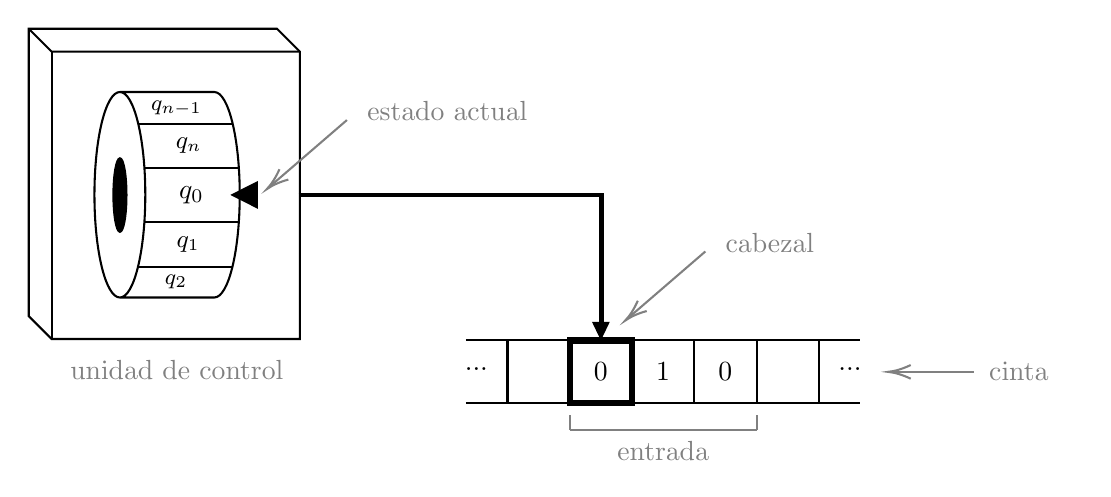
\begin{tikzpicture}[x=0.75pt,y=0.75pt,yscale=-1,xscale=1]
%uncomment if require: \path (0,221); %set diagram left start at 0, and has height of 221

%Flowchart: Direct Access Storage [id:dp5745083904317894] 
\draw   (45.92,32.5) -- (91.42,32.5) .. controls (98.18,32.5) and (103.67,54.66) .. (103.67,82) .. controls (103.67,109.34) and (98.18,131.5) .. (91.42,131.5) -- (45.92,131.5)(33.67,82) .. controls (33.67,54.66) and (39.15,32.5) .. (45.92,32.5) .. controls (52.68,32.5) and (58.17,54.66) .. (58.17,82) .. controls (58.17,109.34) and (52.68,131.5) .. (45.92,131.5) .. controls (39.15,131.5) and (33.67,109.34) .. (33.67,82) ;
%Shape: Cube [id:dp9677041927446011] 
\draw   (132.67,13.07) -- (121.59,2) -- (2,2) -- (2,140.43) -- (13.07,151.5) -- (132.67,151.5) -- cycle ; \draw   (2,2) -- (13.07,13.07) -- (132.67,13.07) ; \draw   (13.07,13.07) -- (13.07,151.5) ;
%Shape: Ellipse [id:dp3944720200277354] 
\draw  [fill={rgb, 255:red, 0; green, 0; blue, 0 }  ,fill opacity=1 ] (42.81,82.14) .. controls (42.81,72.36) and (44.22,64.43) .. (45.95,64.43) .. controls (47.69,64.43) and (49.1,72.36) .. (49.1,82.14) .. controls (49.1,91.93) and (47.69,99.86) .. (45.95,99.86) .. controls (44.22,99.86) and (42.81,91.93) .. (42.81,82.14) -- cycle ;
%Straight Lines [id:da7811026207895715] 
\draw    (57.67,95) -- (103.1,95) ;
%Straight Lines [id:da7715257519556658] 
\draw    (54.52,116.86) -- (99.95,116.86) ;
%Straight Lines [id:da7719478908390764] 
\draw    (55.1,47.86) -- (100.52,47.86) ;
%Straight Lines [id:da44878361199349515] 
\draw    (57.67,69) -- (103.1,69) ;
%Flowchart: Merge [id:dp7750110622325217] 
\draw  [fill={rgb, 255:red, 0; green, 0; blue, 0 }  ,fill opacity=1 ] (111.95,76.14) -- (111.95,88) -- (100.24,82.07) -- cycle ;
%Shape: Rectangle [id:dp3100328904459395] 
\draw   (232.67,152.17) -- (262.67,152.17) -- (262.67,182.17) -- (232.67,182.17) -- cycle ;
%Shape: Rectangle [id:dp1692041741743724] 
\draw  [line width=2.25]  (262.67,152.17) -- (292.67,152.17) -- (292.67,182.17) -- (262.67,182.17) -- cycle ;
%Shape: Rectangle [id:dp5247156403937852] 
\draw   (292.67,152.17) -- (322.67,152.17) -- (322.67,182.17) -- (292.67,182.17) -- cycle ;
%Shape: Rectangle [id:dp1939162798122891] 
\draw   (322.67,152.17) -- (352.67,152.17) -- (352.67,182.17) -- (322.67,182.17) -- cycle ;
%Shape: Rectangle [id:dp955944006123826] 
\draw   (352.67,152.17) -- (382.67,152.17) -- (382.67,182.17) -- (352.67,182.17) -- cycle ;
%Straight Lines [id:da2297213302864911] 
\draw    (382.67,152.17) -- (402.67,152.17) ;
%Straight Lines [id:da0017979141787713981] 
\draw    (382.67,182.17) -- (402.67,182.17) ;
%Straight Lines [id:da5196954519515742] 
\draw    (212.67,182.17) -- (232.67,182.17) ;
%Straight Lines [id:da6250621041798603] 
\draw    (212.67,152.17) -- (232.67,152.17) ;
%Straight Lines [id:da4041928331954272] 
\draw [color={rgb, 255:red, 128; green, 128; blue, 128 }  ,draw opacity=1 ]   (262.67,195.17) -- (352.67,195.17) ;
%Straight Lines [id:da40491651879492707] 
\draw [color={rgb, 255:red, 128; green, 128; blue, 128 }  ,draw opacity=1 ]   (262.67,188.17) -- (262.67,195.17) ;
%Straight Lines [id:da9178129384480556] 
\draw [color={rgb, 255:red, 128; green, 128; blue, 128 }  ,draw opacity=1 ]   (352.67,188.17) -- (352.67,195.17) ;
%Shape: Right Angle [id:dp42415196847546355] 
\draw  [line width=1.5]  (132,82) -- (278,82) -- (278,146) ;
%Straight Lines [id:da05158428581441665] 
\draw    (277.67,128) -- (277.67,149.17) ;
\draw [shift={(277.67,152.17)}, rotate = 270] [fill={rgb, 255:red, 0; green, 0; blue, 0 }  ][line width=0.08]  [draw opacity=0] (8.93,-4.29) -- (0,0) -- (8.93,4.29) -- cycle    ;
%Straight Lines [id:da7132164152395672] 
\draw [color={rgb, 255:red, 128; green, 128; blue, 128 }  ,draw opacity=1 ]   (155.33,46) -- (118.18,78.03) ;
\draw [shift={(116.67,79.33)}, rotate = 319.24] [color={rgb, 255:red, 128; green, 128; blue, 128 }  ,draw opacity=1 ][line width=0.75]    (10.93,-3.29) .. controls (6.95,-1.4) and (3.31,-0.3) .. (0,0) .. controls (3.31,0.3) and (6.95,1.4) .. (10.93,3.29)   ;
%Straight Lines [id:da42945985402945897] 
\draw [color={rgb, 255:red, 128; green, 128; blue, 128 }  ,draw opacity=1 ]   (457.33,167.33) -- (418,167.33) ;
\draw [shift={(416,167.33)}, rotate = 360] [color={rgb, 255:red, 128; green, 128; blue, 128 }  ,draw opacity=1 ][line width=0.75]    (10.93,-3.29) .. controls (6.95,-1.4) and (3.31,-0.3) .. (0,0) .. controls (3.31,0.3) and (6.95,1.4) .. (10.93,3.29)   ;
%Straight Lines [id:da3859416199015755] 
\draw [color={rgb, 255:red, 128; green, 128; blue, 128 }  ,draw opacity=1 ]   (328,109.33) -- (290.85,141.36) ;
\draw [shift={(289.33,142.67)}, rotate = 319.24] [color={rgb, 255:red, 128; green, 128; blue, 128 }  ,draw opacity=1 ][line width=0.75]    (10.93,-3.29) .. controls (6.95,-1.4) and (3.31,-0.3) .. (0,0) .. controls (3.31,0.3) and (6.95,1.4) .. (10.93,3.29)   ;

% Text Node
\draw (73.26,40.18) node  [font=\footnotesize] [align=left] {\begin{minipage}[lt]{24.7pt}\setlength\topsep{0pt}
\begin{center}
$q_{n-1}$
\end{center}

\end{minipage}};
% Text Node
\draw (79.1,58.43) node  [font=\small] [align=left] {\begin{minipage}[lt]{32.64pt}\setlength\topsep{0pt}
\begin{center}
$q_n$
\end{center}

\end{minipage}};
% Text Node
\draw (80.38,82) node  [font=\normalsize] [align=left] {\begin{minipage}[lt]{30.89pt}\setlength\topsep{0pt}
\begin{center}
$q_0$
\end{center}

\end{minipage}};
% Text Node
\draw (78.81,105.93) node  [font=\small] [align=left] {\begin{minipage}[lt]{28.75pt}\setlength\topsep{0pt}
\begin{center}
$q_1$
\end{center}

\end{minipage}};
% Text Node
\draw (72.97,124.18) node  [font=\footnotesize] [align=left] {\begin{minipage}[lt]{25.09pt}\setlength\topsep{0pt}
\begin{center}
$q_2$
\end{center}

\end{minipage}};
% Text Node
\draw (247.67,167.17) node  [font=\normalsize] [align=left] {\begin{minipage}[lt]{20.4pt}\setlength\topsep{0pt}
\begin{center}
\Vtextvisiblespace
\end{center}

\end{minipage}};
% Text Node
\draw (277.67,167.17) node  [font=\normalsize] [align=left] {\begin{minipage}[lt]{20.4pt}\setlength\topsep{0pt}
\begin{center}
$0$
\end{center}

\end{minipage}};
% Text Node
\draw (307.67,167.17) node  [font=\normalsize] [align=left] {\begin{minipage}[lt]{20.4pt}\setlength\topsep{0pt}
\begin{center}
$1$
\end{center}

\end{minipage}};
% Text Node
\draw (337.67,167.17) node  [font=\normalsize] [align=left] {\begin{minipage}[lt]{20.4pt}\setlength\topsep{0pt}
\begin{center}
$0$
\end{center}

\end{minipage}};
% Text Node
\draw (367.67,167.17) node  [font=\normalsize] [align=left] {\begin{minipage}[lt]{20.4pt}\setlength\topsep{0pt}
\begin{center}
\Vtextvisiblespace
\end{center}

\end{minipage}};
% Text Node
\draw (397.67,167.17) node  [font=\normalsize] [align=left] {\begin{minipage}[lt]{20.4pt}\setlength\topsep{0pt}
\begin{center}
$...$
\end{center}

\end{minipage}};
% Text Node
\draw (217.67,167.17) node  [font=\normalsize] [align=left] {\begin{minipage}[lt]{20.4pt}\setlength\topsep{0pt}
\begin{center}
$...$
\end{center}

\end{minipage}};
% Text Node
\draw (307.67,205.17) node  [font=\normalsize,color={rgb, 255:red, 128; green, 128; blue, 128 }  ,opacity=1 ] [align=left] {\begin{minipage}[lt]{61.2pt}\setlength\topsep{0pt}
\begin{center}
entrada
\end{center}

\end{minipage}};
% Text Node
\draw (73.33,166.5) node  [font=\normalsize,color={rgb, 255:red, 128; green, 128; blue, 128 }  ,opacity=1 ] [align=left] {\begin{minipage}[lt]{91.57pt}\setlength\topsep{0pt}
\begin{center}
unidad de control
\end{center}

\end{minipage}};
% Text Node
\draw (214.69,41.83) node  [font=\normalsize,color={rgb, 255:red, 128; green, 128; blue, 128 }  ,opacity=1 ] [align=left] {\begin{minipage}[lt]{74.32pt}\setlength\topsep{0pt}
estado actual
\end{minipage}};
% Text Node
\draw (485.02,167.17) node  [font=\normalsize,color={rgb, 255:red, 128; green, 128; blue, 128 }  ,opacity=1 ] [align=left] {\begin{minipage}[lt]{30.35pt}\setlength\topsep{0pt}
cinta
\end{minipage}};
% Text Node
\draw (387.35,105.17) node  [font=\normalsize,color={rgb, 255:red, 128; green, 128; blue, 128 }  ,opacity=1 ] [align=left] {\begin{minipage}[lt]{74.32pt}\setlength\topsep{0pt}
cabezal
\end{minipage}};


\end{tikzpicture}
\caption{Configuración inicial de una máquina de Turing para la entrada $010$}
\label{fig:maquina-turing}
\end{figure}
% ====================

Es importante aclarar que la máquina de Turing realmente no tiene ninguna ``unidad de control'' o ``cabezal'': es una descripción matemática. Lo que hemos hecho es proporcionar una especificación intuitiva de cómo se ejecuta el algoritmo que representa tal máquina.

Para describir la máquina en cada momento, necesitaremos el concepto de \emph{configuración}.

% ====================
\begin{definicion}[Configuración de una máquina de Turing]\label{def:configuracion-maquina-turing}
\index{configuración}\index{configuración!de una máquina de Turing de una sola cinta}
Especificaremos la \emph{configuración} de una máquina de Turing mediante dos parámetros:

\begin{itemize}
    \item El estado $q\in Q$ en el que se encuentra la máquina.
    \item La palabra $w \in B^*$ presente en la \emph{cinta} y la posición del \emph{cabezal de lectura}, que representaremos recuadrando el símbolo donde se encuentra el cabezal. Dado que el cabezal se extiende infinitamente a ambos lados, eliminamos los caracteres blancos a la izquierda y a la derecha hasta llegar a la posición del cabezal.
\end{itemize}

Representaremos una configuración mediante $$q\;:\;w$$ con uno de los símbolos de $w$ debidamente recuadrado.
\end{definicion}
% ====================

Lo único que nos queda es precisar la noción de ``transición'' que comentamos anteriormente. En cada paso, aplicamos una transición y cambiamos la configuración de la máquina. Esto es lo que denominamos \emph{proceso de cálculo}, y formalizamos a continuación.

% ====================
\begin{definicion}[Proceso de cálculo de una máquina de Turing]\label{def:proceso-calculo-maquina-turing}
\index{proceso de cálculo}\index{proceso de cálculo!de una máquina de Turing de una sola cinta}
Dada una máquina de Turing $M=(Q, A, B, \delta, q_0, \Vtextvisiblespace\:, F)$, y dada una entrada inicial $u = u_1\:u_2\:...\:u_n\in A^*$, definimos su \emph{configuración inicial}\index{configuración!inicial} como:
$$
    q_0\;:\;\fbox{$u_1$}\:u_2\:...\:u_n
$$
A continuación, definimos un \emph{paso de cálculo}  para cada configuración de la máquina:
$$q\;:\;b_{-n}\:...\:b_{-2}\:b_{-1}\:\fbox{$b_0$}\:b_1\:b_2\:...\:b_m$$
con $q\in Q, b=b_{-n}\:...\:b_{-2}\:b_{-1}\:b_0\:b_1\:b_2\:...\:b_m\in B^*$, en función del valor de la función de transición $\delta(q,b)$:
\begin{itemize}
    \item Si $\delta(q,b)$ no está definido $(\delta(q,b)=\emptyset$), la máquina para.
    \item Si $\delta(q,b)=(p,c,M)$ con $p\in Q, c\in B, M\in \{I,D,S\}$, la máquina reemplazará el símbolo $b$ presente en la posición de la cinta en la que se encuentra el cabezal por $c$, moverá el cabezal una posición de acuerdo a $M$ (a la izquierda, derecha o no se moverá si es $I$, $D$ o $S$, respectivamente), y cambiará su estado a $p$:
    $$
        \begin{matrix}
            M=I&\Rightarrow&p\;:\;b_{-n}\:...\:b_{-2}\:\fbox{$b_{-1}$}\:c\:b_1\:b_2\:...\:b_m\\
            M=D&\Rightarrow&p\;:\;b_{-n}\:...\:b_{-2}\:b_{-1}\:c\:\fbox{$b_1$}\:b_2\:...\:b_m\\
            M=S&\Rightarrow&p\;:\;b_{-n}\:...\:b_{-2}\:b_{-1}\:\fbox{$c$}\:b_1\:b_2\:...\:b_m
        \end{matrix}
    $$
\end{itemize}
El \emph{proceso de cálculo} se define como la consecución de pasos de cálculo, comenzando por la configuración inicial.

Es posible que la máquina pare cuando llega a una configuración tal que la función de transición no está definida.\footnote{Nótese que esta definición permite que la máquina siga cambiando su configuración aun habiendo llegado a un estado final. Normalmente, las máquinas de Turing paran llegado al estado final, y esto es algo de lo que nos podemos asegurar simplemente haciendo que $\delta(q,b)=\emptyset\;\forall q\in F, b\in B$.} Si esto no ocurre, la sucesión de pasos de cálculo será infinita y la máquina no parará nunca.
\end{definicion}
% ====================

En definitiva, vemos que la máquina, en función del estado en el que se encuentre y el símbolo escaneado, ejecutará una cierta transición, definida en $\delta$, que le dirá a qué estado pasar, por qué símbolo reemplazar el escaneado y el movimiento que tiene que realizar sobre la cinta.

Una nota importante respecto a las transiciones no definidas. A la hora de describir una función de transición, definiremos únicamente las transiciones para los estados $q\in Q$ y símbolos $b \in B$ para los que están definidas. En caso contrario, podemos asumir que \linebreak $\delta(q, b) = \emptyset$. Puedes ver esto en el \cref{ej:mt-1}, que comentaremos en detalle más adelante.


Introducimos una notación gráfica para la función de transición. La definiremos mediante un grafo dirigido, representaremos los estados como nodos (uno para cada estado) y las transiciones como arcos dirigidos.


El estado inicial se simbolizará, además de en la definición de la máquina, con una flecha apuntando al estado (no es un arco, sino que no proviene de ningún nodo):

% ====================
\begin{center}
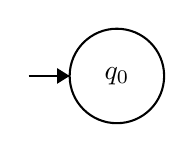
\begin{tikzpicture}[scale=0.2]
\tikzstyle{every node}+=[inner sep=0pt]
\draw [black] (11.8,-27.6) circle (3);
\draw (11.8,-27.6) node {$q_0$};
\draw [black] (6.2,-27.6) -- (8.8,-27.6);
\fill [black] (8.8,-27.6) -- (8,-27.1) -- (8,-28.1);
\end{tikzpicture}
\end{center}
% ====================

Para cada transición $\delta(q,b)=(p,c,M)$, insertaremos un arco dirigido conectando los nodos correspondientes a los estados $q$ y $p$ como sigue:

% ====================
\begin{center}
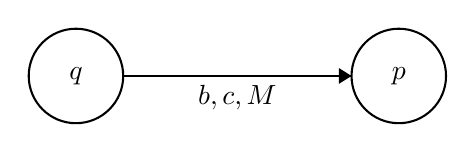
\begin{tikzpicture}[scale=0.2]
\tikzstyle{every node}+=[inner sep=0pt]
\draw [black] (11.8,-27.6) circle (3);
\draw (11.8,-27.6) node {$q$};
\draw [black] (32.3,-27.6) circle (3);
\draw (32.3,-27.6) node {$p$};
\draw [black] (14.8,-27.6) -- (29.3,-27.6);
\fill [black] (29.3,-27.6) -- (28.5,-27.1) -- (28.5,-28.1);
\draw (22.05,-28.1) node [below] {$b,c,M$};
\end{tikzpicture}
\end{center}
% ====================

En caso de que tengamos varias funciones de transición entre ambos estados ($\delta(q,b)=(p,c,M)$ y $\delta(q,b')=(p,c',M')$) colocaremos varias líneas en el arco para simbolizarlo:

% ====================
\begin{center}
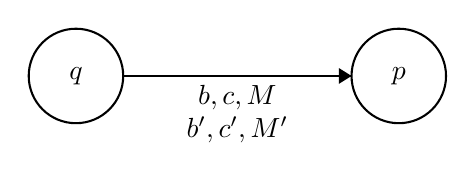
\begin{tikzpicture}[scale=0.2]
\tikzstyle{every node}+=[inner sep=0pt]
\draw [black] (11.8,-27.6) circle (3);
\draw (11.8,-27.6) node {$q$};
\draw [black] (32.3,-27.6) circle (3);
\draw (32.3,-27.6) node {$p$};
\draw [black] (14.8,-27.6) -- (29.3,-27.6);
\fill [black] (29.3,-27.6) -- (28.5,-27.1) -- (28.5,-28.1);
\draw (22.05,-28.1) node [below] {$b,c,M$};
\draw (22.05,-30.1) node [below] {$b',c',M'$};
\end{tikzpicture}
\end{center}
% ====================

Finalmente, también indicaremos los estados finales rodeando dos veces el arco:

% ====================
\begin{center}
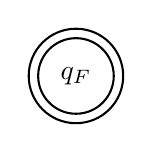
\begin{tikzpicture}[scale=0.2]
\tikzstyle{every node}+=[inner sep=0pt]
\draw [black] (11.8,-27.6) circle (3);
\draw (11.8,-27.6) node {$q_F$};
\draw [black] (11.8,-27.6) circle (2.4);
\end{tikzpicture}
\end{center}
% ====================

Observemos cómo una máquina de Turing, dada una entrada, puede:
\begin{itemize}
    \item parar y aceptar,
    \item parar y rechazar, o
    \item no parar (\emph{ciclar}).\index{ciclar}
\end{itemize}

La máquina para cuando llega a una configuración para la que no hay una transición definida. Cuando ocurre esto, podemos definir una salida con los símbolos que quedan en la cinta.

% ====================
\begin{definicion}[Salida de una máquina de Turing]\label{def:salida-maquina-turing}
\index{salida!de una máquina de Turing}
Para una máquina de Turing $M$, definimos su \emph{salida} como los contenidos de la cinta una vez que la máquina ha parado, omitiendo los símbolos blancos a ambos lados.
\end{definicion}
% ====================

% ====================
\begin{definicion}[Palabra aceptada por una máquina de Turing]\label{def:palabra-aceptada-maquina-turing}
\index{palabra!aceptada por una máquina de Turing}
Dada una máquina de Turing $M=(Q, A, B, \delta, q_0, \Vtextvisiblespace\:, F)$, y dada una entrada inicial $u \in A^*$, decimos que \emph{$M$ acepta $u$} si $M$ para con entrada $u$ en un estado $q\in F$. Si lo hace en un estado $q \notin F$, decimos que \emph{$M$ rechaza $u$}.\index{palabra!rechazada por una máquina de Turing}
\end{definicion}
% ====================

Al haber definido qué palabras acepta una máquina determinada, introducimos el concepto de \emph{lenguaje}.\index{lenguaje} Un lenguaje no es más que un conjunto de palabras.%, por lo que podemos preguntarnos por el lenguaje que acepta una cierta máquina.

% ====================
\begin{definicion}[Lenguaje aceptado por una máquina de Turing]
\index{lenguaje!aceptado por una máquina de Turing}
    Un lenguaje $L$ sobre un alfabeto $A$ es un conjunto de palabras sobre $A$.

    Si $M=(Q, A, B, \delta, q_0, \Vtextvisiblespace\:, F)$ es una máquina de Turing, el \emph{lenguaje aceptado}, denotado como $L(M)$, es el conjunto de palabras aceptadas por $M$, es decir,
    $$
        u\in L(M)\;\iff\;M\text{ acepta }u
    $$
\end{definicion}
% ====================

Concretemos todos los conceptos que hemos introducido mediante un ejemplo.

% ====================
\begin{ejemplo}\label{ej:mt-1}Sea $M_{\#a>\#b}$ una máquina de Turing tal que:
$$
    M_{\#a>\#b}=(\{q_0, q_a, q_b, q_R, q_F\}, \{a, b\}, \{a, b, X, \Vtextvisiblespace\}, \delta, q_0, \Vtextvisiblespace\:,\{q_F\})
$$
con $\delta$, su función de transición, descrita mediante el grafo:
\vfill
% ====================
\begin{figure}[H]
\centering
\resizebox{.7\linewidth}{!}{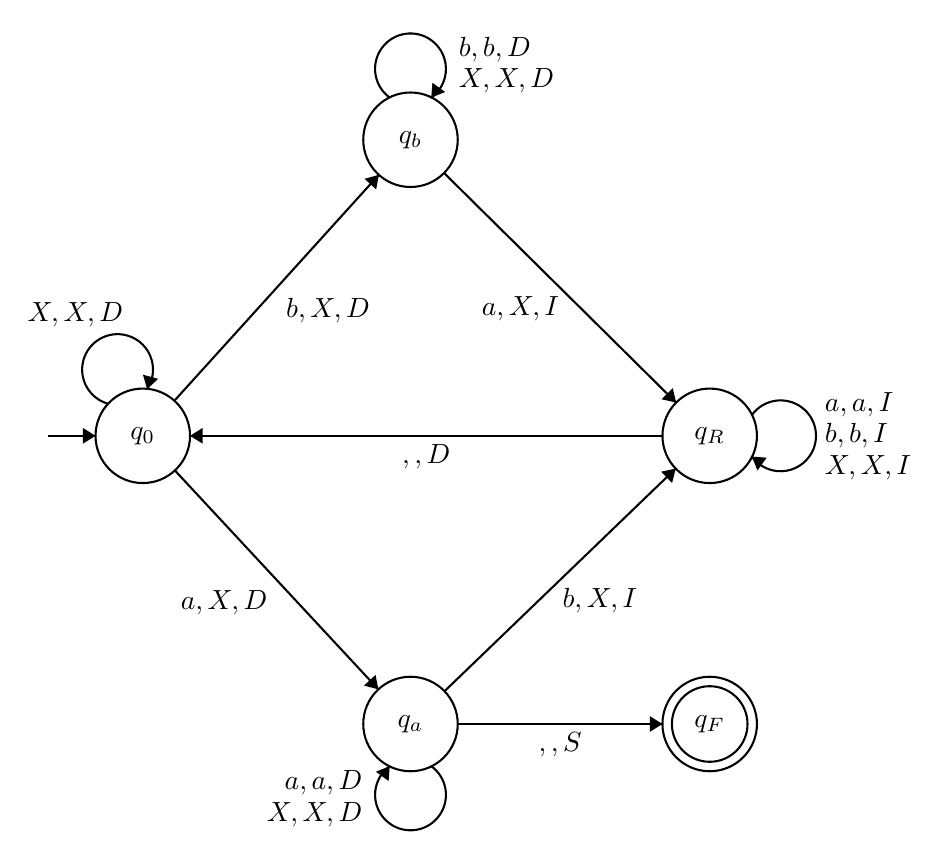
\begin{tikzpicture}[scale=0.2]
\tikzstyle{every node}+=[inner sep=0pt]
\draw [black] (28.8,-27.6) circle (3);
\draw (28.8,-27.6) node {$q_0$};
\draw [black] (64.8,-27.6) circle (3);
\draw (64.8,-27.6) node {$q_R$};
\draw [black] (45.8,-8.8) circle (3);
\draw (45.8,-8.8) node {$q_b$};
\draw [black] (45.8,-45.9) circle (3);
\draw (45.8,-45.9) node {$q_a$};
\draw [black] (64.8,-45.9) circle (3);
\draw (64.8,-45.9) node {$q_F$};
\draw [black] (64.8,-45.9) circle (2.4);
\draw [black] (22.8,-27.6) -- (25.8,-27.6);
\fill [black] (25.8,-27.6) -- (25,-27.1) -- (25,-28.1);
\draw [black] (26.611,-25.566) arc (254.8313:-33.1687:2.25);
\draw (24.52,-20.75) node [above] {$X,X,D$};
\fill [black] (29.08,-24.63) -- (29.78,-23.98) -- (28.81,-23.72);
\draw [black] (31.8,-27.6) -- (61.8,-27.6);
\fill [black] (31.8,-27.6) -- (32.6,-27.1) -- (32.6,-28.1);
\draw (46.8,-28.1) node [below] {$\Vtextvisiblespace, \Vtextvisiblespace, D$};
\draw [black] (30.84,-29.8) -- (43.76,-43.7);
\fill [black] (43.76,-43.7) -- (43.58,-42.78) -- (42.85,-43.46);
\draw (36.77,-38.21) node [left] {$a,X,D$};
\draw [black] (47.96,-43.82) -- (62.64,-29.68);
\fill [black] (62.64,-29.68) -- (61.72,-29.88) -- (62.41,-30.6);
\draw (57.82,-37.23) node [below] {$b,X,I$};
\draw [black] (47.123,-48.58) arc (54:-234:2.25);
\draw (42.8,-49.65) node [left] {$a,a,D$};
\draw (42.8,-51.65) node [left] {$X,X,D$};
\fill [black] (44.48,-48.58) -- (43.6,-48.93) -- (44.41,-49.52);
\draw [black] (44.477,-6.12) arc (234:-54:2.25);
\draw (48.8,-3.05) node [right] {$b,b,D$};
\draw (48.8,-5.05) node [right] {$X,X,D$};
\fill [black] (47.12,-6.12) -- (48,-5.77) -- (47.19,-5.18);
\draw [black] (67.48,-26.277) arc (144:-144:2.25);
\draw (72.05,-25.6) node [right] {$a,a,I$};
\draw (72.05,-27.6) node [right] {$b,b,I$};
\draw (72.05,-29.6) node [right] {$X,X,I$};
\fill [black] (67.48,-28.92) -- (67.83,-29.8) -- (68.42,-28.99);
\draw [black] (30.81,-25.37) -- (43.79,-11.03);
\fill [black] (43.79,-11.03) -- (42.88,-11.28) -- (43.62,-11.95);
\draw (37.84,-19.66) node [right] {$b,X,D$};
\draw [black] (47.93,-10.91) -- (62.67,-25.49);
\fill [black] (62.67,-25.49) -- (62.45,-24.57) -- (61.75,-25.28);
\draw (52.78,-18.68) node [below] {$a,X,I$};
\draw [black] (48.8,-45.9) -- (61.8,-45.9);
\fill [black] (61.8,-45.9) -- (61,-45.4) -- (61,-46.4);
\draw (55.3,-46.4) node [below] {$\Vtextvisiblespace, \Vtextvisiblespace, S$};
\end{tikzpicture}}
\caption{La función de transición $\delta$ de $M_{\#a>\#b}$}
\label{fig:ejemplo-grafo}
\end{figure}
% ====================
\vfill
\pagebreak
Equivalentemente podemos definir la función de transición explícitamente:
$$
    \begin{matrix}
        \delta(q_0, a) = (q_a,X,D) & \delta(q_0, b) = (q_b,X,D) & \delta(q_0, X) = (q_0,X,D) &  \\
        \delta(q_a, a) = (q_a,a,D) & \delta(q_a, b) = (q_R,X,I) & \delta(q_a, X) = (q_a,X,D) & \delta(q_a, \Vtextvisiblespace) = (q_F,\Vtextvisiblespace,S) \\
        \delta(q_b, a) = (q_R,X,I) & \delta(q_b, b) = (q_b,b,D) & \delta(q_b, X) = (q_b,X,D) &  \\
        \delta(q_R, a) = (q_R,a,I) & \delta(q_R, b) = (q_R,b,I) & \delta(q_R, X) = (q_R,X,I) & \delta(q_R, \Vtextvisiblespace) = (q_0,\Vtextvisiblespace,D) \\
    \end{matrix}
$$


Veamos qué hace esta máquina. Empieza al principio de la cinta, y escanea los símbolos uno a uno, de izquierda a derecha. Hay tres posibilidades, dependiendo de si vemos $a$, $b$ o $\Vtextvisiblespace\:$:

\begin{enumerate}
    \item Si se lee una $b$:
        \begin{enumerate}
            \item[1.1.] Reemplazar la $b$ con una $X$.
            \item[1.2.] Continuar escaneando hacia la derecha.
            \begin{enumerate}
                \item[1.2.1.] Si encontramos una $a$, reemplazarla con una $X$. Habremos reemplazado el mismo número de $a$ que de $b$, así que nos movemos al inicio de la cinta y reiniciamos el algoritmo.
                \item[1.2.2.] Si no encontramos una $a$, tenemos una $b$ de más, así que \textit{rechazamos}.
            \end{enumerate}
        \end{enumerate}
    \item Si se lee una $a$:
        \begin{enumerate}
            \item[2.1.] Reemplazar la $a$ con una $X$.
            \item[2.2.] Continuar escaneando hacia la derecha.
            \begin{enumerate}
                \item[2.2.1.] Si encontramos una $b$, reemplazarla con una $X$. Habremos reemplazado el mismo número de $a$ que de $b$, así que nos movemos al inicio de la cinta y reiniciamos el algoritmo.
                \item[2.2.2.] Si no encontramos una $b$, tenemos una $a$ de más, así que \textit{aceptamos}.
            \end{enumerate}
        \end{enumerate}
    \item Si no encontramos $a$ o $b$ antes del $\Vtextvisiblespace$ al final de la entrada: el número de $a$ reemplazados equivale al número de $b$ reemplazados, así que \textit{rechazamos}.
\end{enumerate}


El lenguaje aceptado por esta máquina es el conjunto de palabras de $\{a,b\}^*$ con un número de $a$ mayor que de $b$:\footnote{Usamos la notación: $\#(u, a)$ es igual al número de apariencias del símbolo $a$ en $u$.}
$$
    L(M_{\#a>\#b})=\left\{ u\in\{a,b\}^*\;:\;\#(u,a)>\#(u,b) \right\}
$$
Veamos un ejemplo de palabra aceptada: $abbaa$. Los pasos que da la máquina de Turing configuración tras configuración serán los siguientes:
$$
    \begin{matrix}
        q_0\;:\;\fbox{$a$}\:b\:b\:a\:a & \rightarrow & q_a\;:\;X\:\fbox{$b$}\:b\:a\:a & \rightarrow & q_R\;:\;\fbox{$X$}\:X\:b\:a\:a & \rightarrow & q_R\;:\;\fbox{$\Vtextvisiblespace$}\:X\:X\:b\:a\:a \\
        & \rightarrow & q_0\;:\;\fbox{$X$}\:X\:b\:a\:a & \rightarrow & q_0\;:\;X\:\fbox{$X$}\:b\:a\:a & \rightarrow & q_0\;:\;X\:X\:\fbox{$b$}\:a\:a \\
        & \rightarrow & q_b\;:\;X\:X\:X\:\fbox{$a$}\:a & \rightarrow & q_R\;:\;X\:X\:\fbox{$X$}\:X\:a & \rightarrow & q_R\;:\;X\:\fbox{$X$}\:X\:X\:a \\
        & \rightarrow & q_R\;:\;\fbox{$X$}\:X\:X\:X\:a & \rightarrow & q_R\;:\;\fbox{$\Vtextvisiblespace$}\:X\:X\:X\:X\:a & \rightarrow & q_0\;:\;\:\fbox{$X$}\:X\:X\:X\:a \\
        & \rightarrow & q_0\;:\;\:X\:\fbox{$X$}\:X\:X\:a & \rightarrow & q_0\;:\;\:X\:X\:\fbox{$X$}\:X\:a & \rightarrow & q_0\;:\;\:X\:X\:X\:\fbox{$X$}\:a \\
        & \rightarrow & q_0\;:\;\:X\:X\:X\:X\:\fbox{$a$} & \rightarrow & q_a\;:\;\:X\:X\:X\:X\:X\:\fbox{$\Vtextvisiblespace$} & \rightarrow & q_F\;:\;\:X\:X\:X\:X\:X\:\fbox{$\Vtextvisiblespace$}
    \end{matrix}
$$
Como la máquina para en el estado $q_F\in F$, la palabra es aceptada.

Veamos un ejemplo de una palabra no aceptada, como es $abb$.
$$
    \begin{matrix}
        q_0\;:\;\fbox{$a$}\:b\:b & \rightarrow & q_a\;:\;X\:\fbox{$b$}\:b & \rightarrow & q_R\;:\;\fbox{$X$}\:X\:b & \rightarrow & q_R\;:\;\fbox{$\Vtextvisiblespace$}\:X\:X\:b \\
        & \rightarrow & q_0\;:\;\fbox{$X$}\:X\:b & \rightarrow & q_0\;:\;X\:\fbox{$X$}\:b & \rightarrow & q_0\;:\;X\:X\:\fbox{$b$} \\
        & \rightarrow & q_b\;:\;X\:X\:X\:\fbox{$\Vtextvisiblespace$}
    \end{matrix}
$$
Como la máquina para en el estado $q_b\notin F$, la palabra no es aceptada.

La máquina también permite la entrada vacía ($\epsilon$, que definimos en \cref{def:preliminares}), en cuyo caso la sucesión de configuraciones será:
$$
    \begin{matrix}
        q_0\;:\;\fbox{$\Vtextvisiblespace$}
    \end{matrix}
$$
La máquina para inmediatamente en $q_0\notin F$, y $\epsilon$ no es aceptada. Esto es esperado, pues $\epsilon$ tiene exactamente el mismo número de $a$ que de $b$.

Estos ejemplos quedan resumidos en la \cref{tab:masaqueb-entradas-salidas}, junto con el comportamiento de la máquina para otras palabras. Observa cuándo cada palabra es aceptada, así como el número de transiciones tras los que la máquina para.
\end{ejemplo}
% ====================

Una vez que hemos descrito con precisión qué es una máquina de Turing, procederemos a probar el resultado más importante de este capítulo (el \cref{teo:equivalencia}), que ya anticipamos en la introducción: la equivalencia entre las máquinas de Turing recién expuestas y los programas en Python que definimos en la \cref{sec:programas-python}.

\vfill
% ====================
\begin{tabla}[H]
\begin{table}[H]
\centering
\begin{tabular}{@{}llllcc@{}}
\toprule
Entrada  & Config. inicial & & Config. al parar & ¿Aceptada? & N.º transiciones \\ \midrule
$abbaa$ & $q_0\;:\;\fbox{$a$}\:b\:b\:a\:a$ & $\rightarrow$ & $q_F\;:\;X\:X\:X\:X\:X\:\fbox{$\Vtextvisiblespace$}$ & sí & 18 \\
$abb$ & $q_0\;:\;\fbox{$a$}\:b\:b$ & $\rightarrow$ & $q_b\;:\;X\:X\:X\:\fbox{$\Vtextvisiblespace$}$ & no & 7 \\
$\epsilon$ & $q_0\;:\;\fbox{$\Vtextvisiblespace$}$ & $\rightarrow$ & $q_0\;:\;\fbox{$\Vtextvisiblespace$}$ & no & 0 \\[8pt]
$abab$ & $q_0\;:\;\fbox{$a$}\:b\:a\:b$ & $\rightarrow$ & $q_0\;:\;X\:X\:X\:X\:\fbox{$\Vtextvisiblespace$}$ & no & 16\\
$ababb$ & $q_0\;:\;\fbox{$a$}\:b\:a\:b\:b$ & $\rightarrow$ & $q_b\;:\;X\:X\:X\:X\:X\:\fbox{$\Vtextvisiblespace$}$ & no & 17\\
$ababa$ & $q_0\;:\;\fbox{$a$}\:b\:a\:b\:a$ & $\rightarrow$ & $q_F\;:\;X\:X\:X\:X\:X\:\fbox{$\Vtextvisiblespace$}$ & sí & 18\\
$abaaab$ & $q_0\;:\;\fbox{$a$}\:b\:a\:a\:a\:b$ & $\rightarrow$ & $q_F\;:\;X\:X\:X\:X\:a\:X\:\fbox{$\Vtextvisiblespace$}$ & sí & 23 \\ \bottomrule
\end{tabular}
\end{table}
\vspace*{-8pt}
\caption{Ejemplos del comportamiento de $M_{\#a>\#b}$ con diversas entradas}
\label{tab:masaqueb-entradas-salidas}
\end{tabla}
% ====================
\vfill
\newpage
\section{Equivalencia}\label{sec:equivalencia}

Nuestro objetivo ahora es comprender por qué las máquinas de Turing tienen la misma potencia de cálculo que los programas en Python. Esto quiere decir que los problemas que podemos resolver en ambos son los mismos.\footnote{No introduciremos el concepto de ``problema'' con precisión hasta el \cref{ch:problema-parada} -- por ahora, nos quedaremos con la noción intuitiva de problema, sin mayor explicación.}

Para probar la equivalencia entre ambos modelos de cálculo, recurriremos al concepto de \emph{simulación}.\index{simulación} Es normal para diferentes modelos computacionales simularse unos a otros. Un ejemplo de esto es la máquina virtual de Java (JVM), que es un modelo abstracto capaz de ejecutar cualquier programa en Java. \cite{Evans2018} Otro ejemplo es el sistema operativo Linux, que es capaz de ejecutar la JVM. Por lo tanto, un ordenador Linux es capaz de ejecutar cualquier programa en Java. Esto es posible mediante la cadena de simulaciones:
$$
    \text{Linux} \leadsto \text{JVM} \leadsto \text{programa en Java}
$$
Usamos la notación $A \leadsto B$ para indicar que $A$ simula a $B$. El hecho de que $A$ simule $B$ quiere decir, sencillamente, que es posible realizar el procedimiento de cálculo de $B$ usando exclusivamente el procedimiento de cálculo de $A$.

Procederemos a probar la equivalencia mostrada mediante la cadena de simulaciones que aparece en la \cref{fig:cadena-simulaciones}.

% ===================+
\begin{figure}[H]
\centering
\vspace*{8pt}

\tikzset{every picture/.style={line width=0.75pt}} %set default line width to 0.75pt        

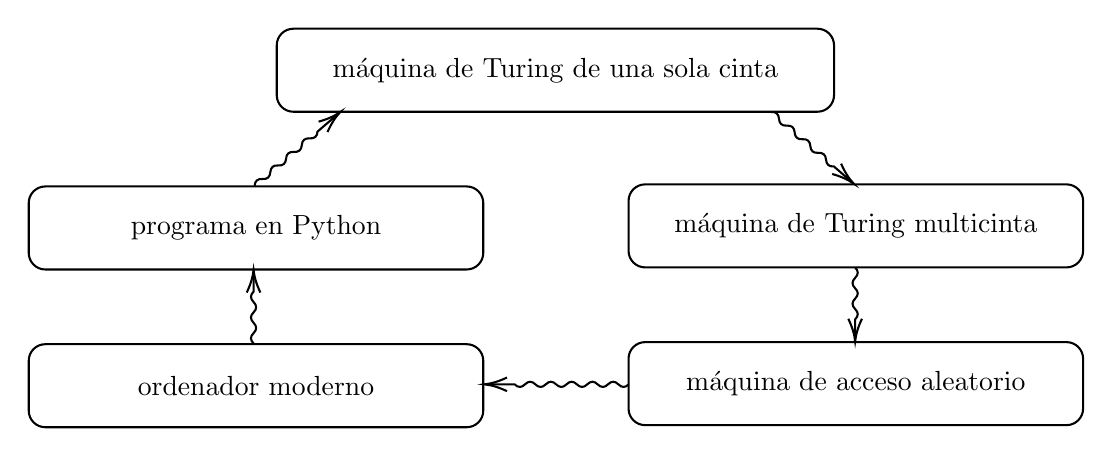
\begin{tikzpicture}[x=0.75pt,y=0.75pt,yscale=-1,xscale=1]
%uncomment if require: \path (0,489); %set diagram left start at 0, and has height of 489

%Rounded Rect [id:dp38098198089187774] 
\draw   (241,29) .. controls (241,24.58) and (244.58,21) .. (249,21) -- (501.5,21) .. controls (505.92,21) and (509.5,24.58) .. (509.5,29) -- (509.5,53) .. controls (509.5,57.42) and (505.92,61) .. (501.5,61) -- (249,61) .. controls (244.58,61) and (241,57.42) .. (241,53) -- cycle ;
%Rounded Rect [id:dp7442940701895104] 
\draw   (410.5,104) .. controls (410.5,99.58) and (414.08,96) .. (418.5,96) -- (621.5,96) .. controls (625.92,96) and (629.5,99.58) .. (629.5,104) -- (629.5,128) .. controls (629.5,132.42) and (625.92,136) .. (621.5,136) -- (418.5,136) .. controls (414.08,136) and (410.5,132.42) .. (410.5,128) -- cycle ;
%Rounded Rect [id:dp05734792720775661] 
\draw   (410.5,180) .. controls (410.5,175.58) and (414.08,172) .. (418.5,172) -- (621.5,172) .. controls (625.92,172) and (629.5,175.58) .. (629.5,180) -- (629.5,204) .. controls (629.5,208.42) and (625.92,212) .. (621.5,212) -- (418.5,212) .. controls (414.08,212) and (410.5,208.42) .. (410.5,204) -- cycle ;
%Rounded Rect [id:dp6203792922315816] 
\draw   (121.5,105) .. controls (121.5,100.58) and (125.08,97) .. (129.5,97) -- (332.5,97) .. controls (336.92,97) and (340.5,100.58) .. (340.5,105) -- (340.5,129) .. controls (340.5,133.42) and (336.92,137) .. (332.5,137) -- (129.5,137) .. controls (125.08,137) and (121.5,133.42) .. (121.5,129) -- cycle ;
%Rounded Rect [id:dp5638157358715545] 
\draw   (121.5,181) .. controls (121.5,176.58) and (125.08,173) .. (129.5,173) -- (332.5,173) .. controls (336.92,173) and (340.5,176.58) .. (340.5,181) -- (340.5,205) .. controls (340.5,209.42) and (336.92,213) .. (332.5,213) -- (129.5,213) .. controls (125.08,213) and (121.5,209.42) .. (121.5,205) -- cycle ;
%Straight Lines [id:da13357301440091862] 
\draw    (479.2,61.14) .. controls (481.55,60.97) and (482.81,62.06) .. (482.98,64.41) .. controls (483.14,66.76) and (484.4,67.86) .. (486.75,67.69) .. controls (489.1,67.52) and (490.36,68.62) .. (490.53,70.97) .. controls (490.7,73.32) and (491.96,74.41) .. (494.31,74.24) .. controls (496.66,74.07) and (497.92,75.17) .. (498.08,77.52) .. controls (498.25,79.87) and (499.51,80.97) .. (501.86,80.8) .. controls (504.21,80.63) and (505.47,81.72) .. (505.64,84.07) .. controls (505.8,86.42) and (507.06,87.52) .. (509.41,87.35) -- (511.45,89.12) -- (517.49,94.36) ;
\draw [shift={(519,95.67)}, rotate = 220.95] [color={rgb, 255:red, 0; green, 0; blue, 0 }  ][line width=0.75]    (10.93,-3.29) .. controls (6.95,-1.4) and (3.31,-0.3) .. (0,0) .. controls (3.31,0.3) and (6.95,1.4) .. (10.93,3.29)   ;
%Straight Lines [id:da7755341344632458] 
\draw    (519.67,136.05) .. controls (521.34,137.72) and (521.34,139.38) .. (519.67,141.05) .. controls (518,142.72) and (518,144.38) .. (519.67,146.05) .. controls (521.34,147.72) and (521.34,149.38) .. (519.67,151.05) .. controls (518,152.72) and (518,154.38) .. (519.67,156.05) .. controls (521.34,157.72) and (521.34,159.38) .. (519.67,161.05) -- (519.67,161.67) -- (519.67,169.67) ;
\draw [shift={(519.67,171.67)}, rotate = 270] [color={rgb, 255:red, 0; green, 0; blue, 0 }  ][line width=0.75]    (10.93,-3.29) .. controls (6.95,-1.4) and (3.31,-0.3) .. (0,0) .. controls (3.31,0.3) and (6.95,1.4) .. (10.93,3.29)   ;
%Straight Lines [id:da5719619240034488] 
\draw    (229.83,172.67) .. controls (228.16,171) and (228.16,169.34) .. (229.83,167.67) .. controls (231.5,166) and (231.5,164.34) .. (229.83,162.67) .. controls (228.16,161) and (228.16,159.34) .. (229.83,157.67) .. controls (231.5,156) and (231.5,154.34) .. (229.83,152.67) .. controls (228.16,151) and (228.16,149.34) .. (229.83,147.67) -- (229.83,147.19) -- (229.83,139.19) ;
\draw [shift={(229.83,137.19)}, rotate = 90] [color={rgb, 255:red, 0; green, 0; blue, 0 }  ][line width=0.75]    (10.93,-3.29) .. controls (6.95,-1.4) and (3.31,-0.3) .. (0,0) .. controls (3.31,0.3) and (6.95,1.4) .. (10.93,3.29)   ;
%Straight Lines [id:da9776591080439316] 
\draw    (410.6,192.34) .. controls (408.93,194.01) and (407.27,194.01) .. (405.6,192.34) .. controls (403.93,190.67) and (402.27,190.67) .. (400.6,192.34) .. controls (398.93,194.01) and (397.27,194.01) .. (395.6,192.34) .. controls (393.93,190.67) and (392.27,190.67) .. (390.6,192.34) .. controls (388.93,194.01) and (387.27,194.01) .. (385.6,192.34) .. controls (383.93,190.67) and (382.27,190.67) .. (380.6,192.34) .. controls (378.93,194.01) and (377.27,194.01) .. (375.6,192.34) .. controls (373.93,190.67) and (372.27,190.67) .. (370.6,192.34) .. controls (368.93,194.01) and (367.27,194.01) .. (365.6,192.34) .. controls (363.93,190.67) and (362.27,190.67) .. (360.6,192.34) .. controls (358.93,194.01) and (357.27,194.01) .. (355.6,192.34) -- (351,192.34) -- (343,192.34) ;
\draw [shift={(341,192.34)}, rotate = 360] [color={rgb, 255:red, 0; green, 0; blue, 0 }  ][line width=0.75]    (10.93,-3.29) .. controls (6.95,-1.4) and (3.31,-0.3) .. (0,0) .. controls (3.31,0.3) and (6.95,1.4) .. (10.93,3.29)   ;
%Straight Lines [id:da4761638716364047] 
\draw    (230.33,96.67) .. controls (230.51,94.32) and (231.77,93.23) .. (234.12,93.41) .. controls (236.47,93.58) and (237.74,92.49) .. (237.91,90.14) .. controls (238.08,87.79) and (239.35,86.7) .. (241.7,86.88) .. controls (244.05,87.06) and (245.32,85.97) .. (245.49,83.62) .. controls (245.66,81.27) and (246.93,80.18) .. (249.28,80.36) .. controls (251.63,80.53) and (252.9,79.44) .. (253.07,77.09) .. controls (253.24,74.74) and (254.51,73.65) .. (256.86,73.83) .. controls (259.21,74.01) and (260.48,72.92) .. (260.65,70.57) -- (264.02,67.66) -- (270.08,62.44) ;
\draw [shift={(271.6,61.14)}, rotate = 139.27] [color={rgb, 255:red, 0; green, 0; blue, 0 }  ][line width=0.75]    (10.93,-3.29) .. controls (6.95,-1.4) and (3.31,-0.3) .. (0,0) .. controls (3.31,0.3) and (6.95,1.4) .. (10.93,3.29)   ;

% Text Node
\draw (375.25,41) node  [font=\normalsize] [align=left] {\begin{minipage}[lt]{171.7pt}\setlength\topsep{0pt}
\begin{center}
máquina de Turing de una sola cinta
\end{center}

\end{minipage}};
% Text Node
\draw (520,116) node  [font=\normalsize] [align=left] {\begin{minipage}[lt]{138.04pt}\setlength\topsep{0pt}
\begin{center}
máquina de Turing multicinta
\end{center}

\end{minipage}};
% Text Node
\draw (520,192) node  [font=\normalsize] [align=left] {\begin{minipage}[lt]{138.04pt}\setlength\topsep{0pt}
\begin{center}
máquina de acceso aleatorio
\end{center}

\end{minipage}};
% Text Node
\draw (231,117) node  [font=\normalsize] [align=left] {\begin{minipage}[lt]{138.04pt}\setlength\topsep{0pt}
\begin{center}
programa en Python
\end{center}

\end{minipage}};
% Text Node
\draw (231,193) node  [font=\normalsize] [align=left] {\begin{minipage}[lt]{138.04pt}\setlength\topsep{0pt}
\begin{center}
ordenador moderno
\end{center}

\end{minipage}};
% Text Node
\draw (551.17,77.84) node  [font=\small] [align=left] {\begin{minipage}[lt]{43.29pt}\setlength\topsep{0pt}
\end{minipage}};
% Text Node
\draw (561.17,153.84) node  [font=\small] [align=left] {\begin{minipage}[lt]{43.29pt}\setlength\topsep{0pt}
\end{minipage}};
% Text Node
\draw (375.8,177.5) node  [font=\small] [align=left] {\begin{minipage}[lt]{47.33pt}\setlength\topsep{0pt}
\begin{center}
\end{center}

\end{minipage}};
% Text Node
\draw (189.67,154.84) node  [font=\small] [align=left] {\begin{minipage}[lt]{43.29pt}\setlength\topsep{0pt}
\begin{flushright}
\end{flushright}

\end{minipage}};
% Text Node
\draw (199.67,78.84) node  [font=\small] [align=left] {\begin{minipage}[lt]{43.29pt}\setlength\topsep{0pt}
\begin{flushright}
\end{flushright}

\end{minipage}};


\end{tikzpicture}
\caption{Cadena de simulaciones}
\label{fig:cadena-simulaciones}
\end{figure}
% ===================+

El trabajo que haremos en esta sección es arduo, y necesitaremos introducir diversos modelos computacionales para llegar a nuestro objetivo. Sin embargo, una vez probemos todas las simulaciones, sabremos que todas ellas son equivalentes, y podremos usar el modelo que queramos a conveniencia.

El primer modelo computacional que estudiaremos lo obtendremos añadiendo más cintas y cabezales a la máquina de Turing que definimos en la \cref{sec:maquinas-turing}. \cite{Sipser2012}

% ===================+
\begin{definicion}[Máquina de Turing multicinta]\label{def:maquina-turing-multicinta}
\index{máquina de Turing!multicinta}
Una \emph{máquina de Turing multicinta} con $k$ cintas es una máquina de Turing convencional en la que tenemos $k$ cintas y $k$ cabezales de lectura. En este sentido, la configuración de una máquina de Turing multicinta\index{configuración!de una máquina de Turing multicinta} se describe como:
$$
    q\;:\;w_1\;,\;w_2\;,\;...\;,\;w_k
$$
donde cada una de las palabras de la cinta tiene uno de sus símbolos recuadrados, simbolizando la posición del cabezal en cada cinta.

La función $\delta : Q \times B^k \longrightarrow \left(Q \times (B \times \{I, D, S\})^k\right) \cup \emptyset$ será de la forma:
$$
\delta(q, b_1, b_2, ..., b_k) = \emptyset
$$
para las transiciones no definidas, y para las definidas:
\begin{multline}
    \delta(q, b_1, b_2, ..., b_k) = (p, c_1, M_1, c_2, M_2, ..., c_k, M_k),\\ \text{ con }q,p\in Q, b_i, c_i \in B, M_i \in \{I, D, S\},\;\forall i \in \{1, 2, ..., k\}
\end{multline}
El proceso de cálculo\index{proceso de cálculo!de una máquina de Turing multicinta} será análogo al de una máquina de Turing de una sola cinta, teniendo $\delta$ en cuenta que el símbolo $b_i$ es el leído por el cabezal $i$-ésimo, que $c_i$ es el símbolo por el que se cambia $b_i$ en el cabezal $i$-ésimo, y $M_i$ es el movimiento que seguirá el cabezal $i$-ésimo.

La entrada de la máquina se colocará en la primera cinta, con el cabezal en el primer símbolo de la palabra. El resto de cabezales apuntarán al símbolo vacío, dado que todas las cintas excepto la primera estarán llenas de símbolos vacíos.

Las palabras aceptadas por la máquina procederán de forma análoga al caso de una sola cinta, teniendo en cuenta si el estado donde la máquina para es final o no (está en $F$).
\end{definicion}
% ===================+

% ===================+
\begin{figure}[H]
\centering
\tikzset{every picture/.style={line width=0.75pt}} %set default line width to 0.75pt        

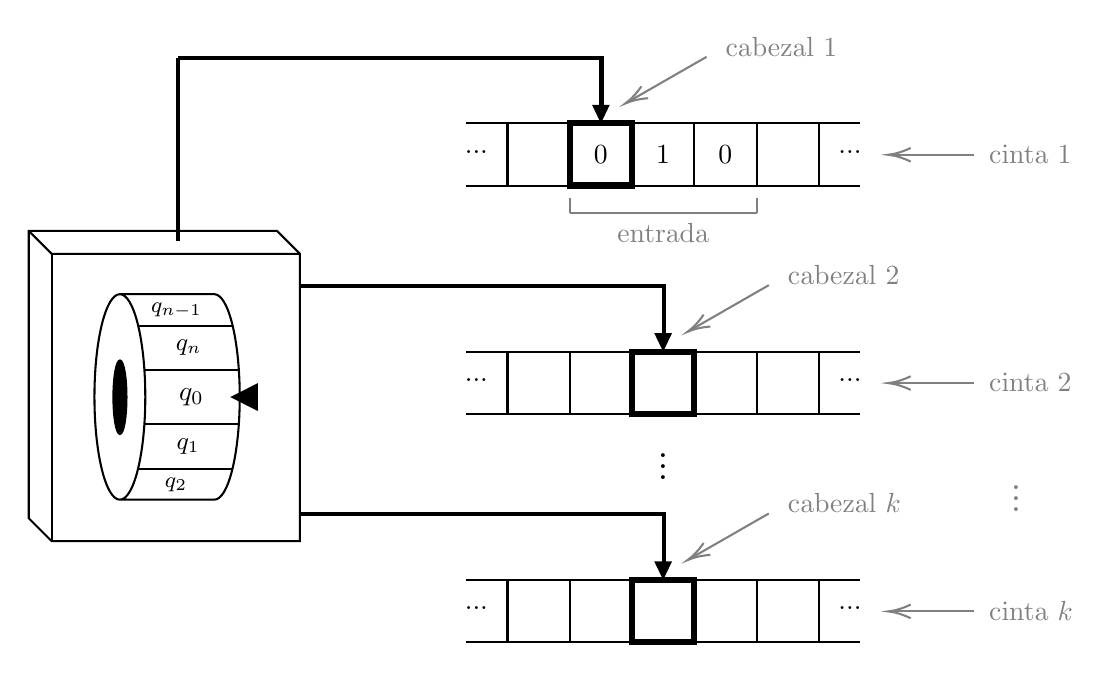
\begin{tikzpicture}[x=0.75pt,y=0.75pt,yscale=-1,xscale=1]
%uncomment if require: \path (0,489); %set diagram left start at 0, and has height of 489

%Flowchart: Direct Access Storage [id:dp884324019015587] 
\draw   (45.92,234.5) -- (91.42,234.5) .. controls (98.18,234.5) and (103.67,256.66) .. (103.67,284) .. controls (103.67,311.34) and (98.18,333.5) .. (91.42,333.5) -- (45.92,333.5)(33.67,284) .. controls (33.67,256.66) and (39.15,234.5) .. (45.92,234.5) .. controls (52.68,234.5) and (58.17,256.66) .. (58.17,284) .. controls (58.17,311.34) and (52.68,333.5) .. (45.92,333.5) .. controls (39.15,333.5) and (33.67,311.34) .. (33.67,284) ;
%Shape: Cube [id:dp11038740716792161] 
\draw   (132.67,215.07) -- (121.59,204) -- (2,204) -- (2,342.43) -- (13.07,353.5) -- (132.67,353.5) -- cycle ; \draw   (2,204) -- (13.07,215.07) -- (132.67,215.07) ; \draw   (13.07,215.07) -- (13.07,353.5) ;
%Shape: Ellipse [id:dp7987859483620612] 
\draw  [fill={rgb, 255:red, 0; green, 0; blue, 0 }  ,fill opacity=1 ] (42.81,284.14) .. controls (42.81,274.36) and (44.22,266.43) .. (45.95,266.43) .. controls (47.69,266.43) and (49.1,274.36) .. (49.1,284.14) .. controls (49.1,293.93) and (47.69,301.86) .. (45.95,301.86) .. controls (44.22,301.86) and (42.81,293.93) .. (42.81,284.14) -- cycle ;
%Straight Lines [id:da9255359456017331] 
\draw    (57.67,297) -- (103.1,297) ;
%Straight Lines [id:da07784762396308076] 
\draw    (54.52,318.86) -- (99.95,318.86) ;
%Straight Lines [id:da9665058890508329] 
\draw    (55.1,249.86) -- (100.52,249.86) ;
%Straight Lines [id:da6649349102379074] 
\draw    (57.67,271) -- (103.1,271) ;
%Flowchart: Merge [id:dp6520009020976827] 
\draw  [fill={rgb, 255:red, 0; green, 0; blue, 0 }  ,fill opacity=1 ] (111.95,278.14) -- (111.95,290) -- (100.24,284.07) -- cycle ;
%Shape: Rectangle [id:dp1739634426056924] 
\draw   (232.67,152.17) -- (262.67,152.17) -- (262.67,182.17) -- (232.67,182.17) -- cycle ;
%Shape: Rectangle [id:dp9225576400306199] 
\draw  [line width=2.25]  (262.67,152.17) -- (292.67,152.17) -- (292.67,182.17) -- (262.67,182.17) -- cycle ;
%Shape: Rectangle [id:dp3089560939474578] 
\draw   (292.67,152.17) -- (322.67,152.17) -- (322.67,182.17) -- (292.67,182.17) -- cycle ;
%Shape: Rectangle [id:dp07530113332493626] 
\draw   (322.67,152.17) -- (352.67,152.17) -- (352.67,182.17) -- (322.67,182.17) -- cycle ;
%Shape: Rectangle [id:dp6187052438945799] 
\draw   (352.67,152.17) -- (382.67,152.17) -- (382.67,182.17) -- (352.67,182.17) -- cycle ;
%Straight Lines [id:da585858356613346] 
\draw    (382.67,152.17) -- (402.67,152.17) ;
%Straight Lines [id:da4527917469159395] 
\draw    (382.67,182.17) -- (402.67,182.17) ;
%Straight Lines [id:da34867855874918985] 
\draw    (212.67,182.17) -- (232.67,182.17) ;
%Straight Lines [id:da2142191065937804] 
\draw    (212.67,152.17) -- (232.67,152.17) ;
%Straight Lines [id:da13729838127645233] 
\draw [color={rgb, 255:red, 128; green, 128; blue, 128 }  ,draw opacity=1 ]   (262.67,195.17) -- (352.67,195.17) ;
%Straight Lines [id:da5262295693466785] 
\draw [color={rgb, 255:red, 128; green, 128; blue, 128 }  ,draw opacity=1 ]   (262.67,188.17) -- (262.67,195.17) ;
%Straight Lines [id:da9629997401870294] 
\draw [color={rgb, 255:red, 128; green, 128; blue, 128 }  ,draw opacity=1 ]   (352.67,188.17) -- (352.67,195.17) ;
%Shape: Right Angle [id:dp20860710988679299] 
\draw  [line width=1.5]  (73.75,120.59) -- (278,120.59) -- (278,146) ;
%Straight Lines [id:da09172139531264967] 
\draw    (277.67,128) -- (277.67,149.17) ;
\draw [shift={(277.67,152.17)}, rotate = 270] [fill={rgb, 255:red, 0; green, 0; blue, 0 }  ][line width=0.08]  [draw opacity=0] (8.93,-4.29) -- (0,0) -- (8.93,4.29) -- cycle    ;
%Straight Lines [id:da8704150337015968] 
\draw [color={rgb, 255:red, 128; green, 128; blue, 128 }  ,draw opacity=1 ]   (457.33,167.33) -- (418,167.33) ;
\draw [shift={(416,167.33)}, rotate = 360] [color={rgb, 255:red, 128; green, 128; blue, 128 }  ,draw opacity=1 ][line width=0.75]    (10.93,-3.29) .. controls (6.95,-1.4) and (3.31,-0.3) .. (0,0) .. controls (3.31,0.3) and (6.95,1.4) .. (10.93,3.29)   ;
%Straight Lines [id:da2111311716419162] 
\draw [color={rgb, 255:red, 128; green, 128; blue, 128 }  ,draw opacity=1 ]   (328.6,120.14) -- (291.07,141.67) ;
\draw [shift={(289.33,142.67)}, rotate = 330.16] [color={rgb, 255:red, 128; green, 128; blue, 128 }  ,draw opacity=1 ][line width=0.75]    (10.93,-3.29) .. controls (6.95,-1.4) and (3.31,-0.3) .. (0,0) .. controls (3.31,0.3) and (6.95,1.4) .. (10.93,3.29)   ;
%Shape: Rectangle [id:dp7885738981424171] 
\draw   (232.67,262.17) -- (262.67,262.17) -- (262.67,292.17) -- (232.67,292.17) -- cycle ;
%Shape: Rectangle [id:dp914560230467196] 
\draw  [line width=0.75]  (262.67,262.17) -- (292.67,262.17) -- (292.67,292.17) -- (262.67,292.17) -- cycle ;
%Shape: Rectangle [id:dp93336651337164] 
\draw  [line width=2.25]  (292.67,262.17) -- (322.67,262.17) -- (322.67,292.17) -- (292.67,292.17) -- cycle ;
%Shape: Rectangle [id:dp6066177634543981] 
\draw   (322.67,262.17) -- (352.67,262.17) -- (352.67,292.17) -- (322.67,292.17) -- cycle ;
%Shape: Rectangle [id:dp29548969777415923] 
\draw   (352.67,262.17) -- (382.67,262.17) -- (382.67,292.17) -- (352.67,292.17) -- cycle ;
%Straight Lines [id:da8417842423391388] 
\draw    (382.67,262.17) -- (402.67,262.17) ;
%Straight Lines [id:da6929186795483306] 
\draw    (382.67,292.17) -- (402.67,292.17) ;
%Straight Lines [id:da33234467498649467] 
\draw    (212.67,292.17) -- (232.67,292.17) ;
%Straight Lines [id:da5040313478090528] 
\draw    (212.67,262.17) -- (232.67,262.17) ;
%Straight Lines [id:da7140976160735828] 
\draw [color={rgb, 255:red, 128; green, 128; blue, 128 }  ,draw opacity=1 ]   (457.33,277.33) -- (418,277.33) ;
\draw [shift={(416,277.33)}, rotate = 360] [color={rgb, 255:red, 128; green, 128; blue, 128 }  ,draw opacity=1 ][line width=0.75]    (10.93,-3.29) .. controls (6.95,-1.4) and (3.31,-0.3) .. (0,0) .. controls (3.31,0.3) and (6.95,1.4) .. (10.93,3.29)   ;
%Shape: Rectangle [id:dp9244189115023447] 
\draw   (232.67,372.17) -- (262.67,372.17) -- (262.67,402.17) -- (232.67,402.17) -- cycle ;
%Shape: Rectangle [id:dp3852380004540896] 
\draw  [line width=0.75]  (262.67,372.17) -- (292.67,372.17) -- (292.67,402.17) -- (262.67,402.17) -- cycle ;
%Shape: Rectangle [id:dp6908829505076823] 
\draw  [line width=2.25]  (292.67,372.17) -- (322.67,372.17) -- (322.67,402.17) -- (292.67,402.17) -- cycle ;
%Shape: Rectangle [id:dp49106618015078873] 
\draw   (322.67,372.17) -- (352.67,372.17) -- (352.67,402.17) -- (322.67,402.17) -- cycle ;
%Shape: Rectangle [id:dp41945989711331855] 
\draw   (352.67,372.17) -- (382.67,372.17) -- (382.67,402.17) -- (352.67,402.17) -- cycle ;
%Straight Lines [id:da5143373708645831] 
\draw    (382.67,372.17) -- (402.67,372.17) ;
%Straight Lines [id:da03282068701218943] 
\draw    (382.67,402.17) -- (402.67,402.17) ;
%Straight Lines [id:da7541958442303496] 
\draw    (212.67,402.17) -- (232.67,402.17) ;
%Straight Lines [id:da3759944034779503] 
\draw    (212.67,372.17) -- (232.67,372.17) ;
%Straight Lines [id:da5842350287046914] 
\draw [color={rgb, 255:red, 128; green, 128; blue, 128 }  ,draw opacity=1 ]   (457.33,387.33) -- (418,387.33) ;
\draw [shift={(416,387.33)}, rotate = 360] [color={rgb, 255:red, 128; green, 128; blue, 128 }  ,draw opacity=1 ][line width=0.75]    (10.93,-3.29) .. controls (6.95,-1.4) and (3.31,-0.3) .. (0,0) .. controls (3.31,0.3) and (6.95,1.4) .. (10.93,3.29)   ;
%Straight Lines [id:da6293362656711181] 
\draw [line width=1.5]    (73.75,120.59) -- (73.75,208.94) ;
%Shape: Right Angle [id:dp7218431782224015] 
\draw  [line width=1.5]  (133,230.59) -- (308,230.59) -- (308,256) ;
%Straight Lines [id:da5357937225858898] 
\draw    (307.67,238) -- (307.67,259.17) ;
\draw [shift={(307.67,262.17)}, rotate = 270] [fill={rgb, 255:red, 0; green, 0; blue, 0 }  ][line width=0.08]  [draw opacity=0] (8.93,-4.29) -- (0,0) -- (8.93,4.29) -- cycle    ;
%Shape: Right Angle [id:dp7257296976920635] 
\draw  [line width=1.5]  (132.43,340.59) -- (308,340.59) -- (308,366) ;
%Straight Lines [id:da5180890057297898] 
\draw    (307.67,348) -- (307.67,369.17) ;
\draw [shift={(307.67,372.17)}, rotate = 270] [fill={rgb, 255:red, 0; green, 0; blue, 0 }  ][line width=0.08]  [draw opacity=0] (8.93,-4.29) -- (0,0) -- (8.93,4.29) -- cycle    ;
%Straight Lines [id:da5847467835308082] 
\draw [color={rgb, 255:red, 128; green, 128; blue, 128 }  ,draw opacity=1 ]   (358.6,230.14) -- (321.07,251.67) ;
\draw [shift={(319.33,252.67)}, rotate = 330.16] [color={rgb, 255:red, 128; green, 128; blue, 128 }  ,draw opacity=1 ][line width=0.75]    (10.93,-3.29) .. controls (6.95,-1.4) and (3.31,-0.3) .. (0,0) .. controls (3.31,0.3) and (6.95,1.4) .. (10.93,3.29)   ;
%Straight Lines [id:da7885667541395345] 
\draw [color={rgb, 255:red, 128; green, 128; blue, 128 }  ,draw opacity=1 ]   (358.6,340.14) -- (321.07,361.67) ;
\draw [shift={(319.33,362.67)}, rotate = 330.16] [color={rgb, 255:red, 128; green, 128; blue, 128 }  ,draw opacity=1 ][line width=0.75]    (10.93,-3.29) .. controls (6.95,-1.4) and (3.31,-0.3) .. (0,0) .. controls (3.31,0.3) and (6.95,1.4) .. (10.93,3.29)   ;

% Text Node
\draw (73.26,242.18) node  [font=\footnotesize] [align=left] {\begin{minipage}[lt]{24.7pt}\setlength\topsep{0pt}
\begin{center}
$q_{n-1}$
\end{center}

\end{minipage}};
% Text Node
\draw (79.1,260.43) node  [font=\small] [align=left] {\begin{minipage}[lt]{32.64pt}\setlength\topsep{0pt}
\begin{center}
$q_n$
\end{center}

\end{minipage}};
% Text Node
\draw (80.38,284) node  [font=\normalsize] [align=left] {\begin{minipage}[lt]{30.89pt}\setlength\topsep{0pt}
\begin{center}
$q_0$
\end{center}

\end{minipage}};
% Text Node
\draw (78.81,307.93) node  [font=\small] [align=left] {\begin{minipage}[lt]{28.75pt}\setlength\topsep{0pt}
\begin{center}
$q_1$
\end{center}

\end{minipage}};
% Text Node
\draw (72.97,326.18) node  [font=\footnotesize] [align=left] {\begin{minipage}[lt]{25.09pt}\setlength\topsep{0pt}
\begin{center}
$q_2$
\end{center}

\end{minipage}};
% Text Node
\draw (247.67,167.17) node  [font=\normalsize] [align=left] {\begin{minipage}[lt]{20.4pt}\setlength\topsep{0pt}
\begin{center}
\Vtextvisiblespace
\end{center}

\end{minipage}};
% Text Node
\draw (277.67,167.17) node  [font=\normalsize] [align=left] {\begin{minipage}[lt]{20.4pt}\setlength\topsep{0pt}
\begin{center}
$0$
\end{center}

\end{minipage}};
% Text Node
\draw (307.67,167.17) node  [font=\normalsize] [align=left] {\begin{minipage}[lt]{20.4pt}\setlength\topsep{0pt}
\begin{center}
$1$
\end{center}

\end{minipage}};
% Text Node
\draw (337.67,167.17) node  [font=\normalsize] [align=left] {\begin{minipage}[lt]{20.4pt}\setlength\topsep{0pt}
\begin{center}
$0$
\end{center}

\end{minipage}};
% Text Node
\draw (367.67,167.17) node  [font=\normalsize] [align=left] {\begin{minipage}[lt]{20.4pt}\setlength\topsep{0pt}
\begin{center}
\Vtextvisiblespace
\end{center}

\end{minipage}};
% Text Node
\draw (397.67,167.17) node  [font=\normalsize] [align=left] {\begin{minipage}[lt]{20.4pt}\setlength\topsep{0pt}
\begin{center}
$...$
\end{center}

\end{minipage}};
% Text Node
\draw (217.67,167.17) node  [font=\normalsize] [align=left] {\begin{minipage}[lt]{20.4pt}\setlength\topsep{0pt}
\begin{center}
$...$
\end{center}

\end{minipage}};
% Text Node
\draw (307.67,205.17) node  [font=\normalsize,color={rgb, 255:red, 128; green, 128; blue, 128 }  ,opacity=1 ] [align=left] {\begin{minipage}[lt]{61.2pt}\setlength\topsep{0pt}
\begin{center}
entrada
\end{center}

\end{minipage}};
% Text Node
\draw (485.02,167.17) node  [font=\normalsize,color={rgb, 255:red, 128; green, 128; blue, 128 }  ,opacity=1 ] [align=left] {\begin{minipage}[lt]{30.35pt}\setlength\topsep{0pt}
cinta $1$
\end{minipage}};
% Text Node
\draw (387.35,115.17) node  [font=\normalsize,color={rgb, 255:red, 128; green, 128; blue, 128 }  ,opacity=1 ] [align=left] {\begin{minipage}[lt]{74.32pt}\setlength\topsep{0pt}
cabezal $1$
\end{minipage}};
% Text Node
\draw (247.67,277.17) node  [font=\normalsize] [align=left] {\begin{minipage}[lt]{20.4pt}\setlength\topsep{0pt}
\begin{center}
\Vtextvisiblespace
\end{center}

\end{minipage}};
% Text Node
\draw (277.67,277.17) node  [font=\normalsize] [align=left] {\begin{minipage}[lt]{20.4pt}\setlength\topsep{0pt}
\begin{center}
\Vtextvisiblespace
\end{center}

\end{minipage}};
% Text Node
\draw (307.67,277.17) node  [font=\normalsize] [align=left] {\begin{minipage}[lt]{20.4pt}\setlength\topsep{0pt}
\begin{center}
\Vtextvisiblespace
\end{center}

\end{minipage}};
% Text Node
\draw (337.67,277.17) node  [font=\normalsize] [align=left] {\begin{minipage}[lt]{20.4pt}\setlength\topsep{0pt}
\begin{center}
\Vtextvisiblespace
\end{center}

\end{minipage}};
% Text Node
\draw (367.67,277.17) node  [font=\normalsize] [align=left] {\begin{minipage}[lt]{20.4pt}\setlength\topsep{0pt}
\begin{center}
\Vtextvisiblespace
\end{center}

\end{minipage}};
% Text Node
\draw (397.67,277.17) node  [font=\normalsize] [align=left] {\begin{minipage}[lt]{20.4pt}\setlength\topsep{0pt}
\begin{center}
$...$
\end{center}

\end{minipage}};
% Text Node
\draw (217.67,277.17) node  [font=\normalsize] [align=left] {\begin{minipage}[lt]{20.4pt}\setlength\topsep{0pt}
\begin{center}
$...$
\end{center}

\end{minipage}};
% Text Node
\draw (485.02,277.17) node  [font=\normalsize,color={rgb, 255:red, 128; green, 128; blue, 128 }  ,opacity=1 ] [align=left] {\begin{minipage}[lt]{30.35pt}\setlength\topsep{0pt}
cinta $2$
\end{minipage}};
% Text Node
\draw (247.67,387.17) node  [font=\normalsize] [align=left] {\begin{minipage}[lt]{20.4pt}\setlength\topsep{0pt}
\begin{center}
\Vtextvisiblespace
\end{center}

\end{minipage}};
% Text Node
\draw (277.67,387.17) node  [font=\normalsize] [align=left] {\begin{minipage}[lt]{20.4pt}\setlength\topsep{0pt}
\begin{center}
\Vtextvisiblespace
\end{center}

\end{minipage}};
% Text Node
\draw (307.67,387.17) node  [font=\normalsize] [align=left] {\begin{minipage}[lt]{20.4pt}\setlength\topsep{0pt}
\begin{center}
\Vtextvisiblespace
\end{center}

\end{minipage}};
% Text Node
\draw (337.67,387.17) node  [font=\normalsize] [align=left] {\begin{minipage}[lt]{20.4pt}\setlength\topsep{0pt}
\begin{center}
\Vtextvisiblespace
\end{center}

\end{minipage}};
% Text Node
\draw (367.67,387.17) node  [font=\normalsize] [align=left] {\begin{minipage}[lt]{20.4pt}\setlength\topsep{0pt}
\begin{center}
\Vtextvisiblespace
\end{center}

\end{minipage}};
% Text Node
\draw (397.67,387.17) node  [font=\normalsize] [align=left] {\begin{minipage}[lt]{20.4pt}\setlength\topsep{0pt}
\begin{center}
$...$
\end{center}

\end{minipage}};
% Text Node
\draw (217.67,387.17) node  [font=\normalsize] [align=left] {\begin{minipage}[lt]{20.4pt}\setlength\topsep{0pt}
\begin{center}
$...$
\end{center}

\end{minipage}};
% Text Node
\draw (485.02,387.17) node  [font=\normalsize,color={rgb, 255:red, 128; green, 128; blue, 128 }  ,opacity=1 ] [align=left] {\begin{minipage}[lt]{30.35pt}\setlength\topsep{0pt}
cinta $k$
\end{minipage}};
% Text Node
\draw (477.67,329.17) node  [font=\Large,color={rgb, 255:red, 128; green, 128; blue, 128 }  ,opacity=1 ] [align=left] {\begin{minipage}[lt]{20.4pt}\setlength\topsep{0pt}
\begin{center}
$\vdots$
\end{center}

\end{minipage}};
% Text Node
\draw (417.35,225.17) node  [font=\normalsize,color={rgb, 255:red, 128; green, 128; blue, 128 }  ,opacity=1 ] [align=left] {\begin{minipage}[lt]{74.32pt}\setlength\topsep{0pt}
cabezal $2$
\end{minipage}};
% Text Node
\draw (417.35,335.17) node  [font=\normalsize,color={rgb, 255:red, 128; green, 128; blue, 128 }  ,opacity=1 ] [align=left] {\begin{minipage}[lt]{74.32pt}\setlength\topsep{0pt}
cabezal $k$
\end{minipage}};
% Text Node
\draw (307.63,313.35) node  [font=\Large,color={rgb, 255:red, 0; green, 0; blue, 0 }  ,opacity=1 ] [align=left] {\begin{minipage}[lt]{20.35pt}\setlength\topsep{0pt}
\begin{center}
$\vdots$
\end{center}

\end{minipage}};


\end{tikzpicture}

\caption{Diagrama de una máquina de Turing multicinta en su configuración inicial}
\label{fig:maquina-turing-multicinta}
\end{figure}
% ===================+

Esta definición es intuitiva y esperable. Simplemente incorporamos más cintas y cabezales. De ahora en adelante, también usaremos el término ``máquina de Turing de una sola cinta'' para referirnos a la máquina de Turing que definimos en primer lugar.

Uno puede pensar que estas máquinas tienen más poder computacional que las de una sola cinta, pero, sin embargo, son equivalentes. Es evidente que una máquina multicinta simula una máquina de una sola cinta (la \cref{def:maquina-turing} es la misma que la \cref{def:maquina-turing-multicinta} para $k=1$). En la \cref{prop:monocinta-a-multicinta} vemos cómo el recíproco también es cierto.

% ===================+
\begin{proposicion}\label{prop:monocinta-a-multicinta}
Toda máquina de Turing multicinta puede ser simulada por una máquina de Turing de una sola cinta.
\end{proposicion}
\begin{proofw}
\emph{Demostración.}\footnote{Basada en la demostración del teorema 3.13 de \cite{Sipser2012}.}$\;\;$Sea $M=(Q, A, B, \delta, q_0, \Vtextvisiblespace\:, F)$ una máquina de Turing con $k$ cintas. Vamos a crear una máquina $\widetilde{M}=(\widetilde{Q}, A, \widetilde{B}, \widetilde{\delta}, q_0, [\Vtextvisiblespace^k]\:, F)$ con una sola cinta de modo que $L(M)=L(\widetilde{M})$. 

Para simular $k$ cintas y $k$ cabezales en un solo cabezal y una sola cinta, deberemos ampliar el alfabeto de trabajo $\widetilde{B}$. En primer lugar, vamos a introducir nuevos símbolos para poder saber la posición de cada uno de los cabezales. Definimos:
$$
    \widecheck{B}=\{\widecheck{b}:b\in B\}
$$
Y, hecho esto, definimos $\widetilde{B}$, el alfabeto de $\widetilde{M}$, como:
$$
    \widetilde{B}=\{[b_1\:b_2\:...\:b_k]:b\in B\cup\widecheck{B}\}\cup\{\#\}
$$
Observemos que los símbolos de $\widetilde{B}$ son bien un delimitador $\#$, bien un grupo de caracteres de $B\cup\widetilde{B}$. De este modo, podemos simular $k$ cintas y $k$ cabezales en una sola cinta con un solo cabezal. Un ejemplo: si en $M$ tenemos la configuración:
$$
    q\;:\;0\:\fbox{$1$}\:0\;,\;X\:X\:\fbox{$X$}\;,\;\fbox{$Y$}\:X
$$
Una de las posibles configuraciones en $\widetilde{M}$ sería:
$$
    q\;:\;\fbox{\#}\:[0\:X\:\widecheck{Y}]\:[\widecheck{1}\:X\:X]\:[0\:\widecheck{X}\:\Vtextvisiblespace]\:\#
$$

% ===================+

% ===================+
\begin{figure}[H]
\centering
\vspace*{8pt}

\tikzset{every picture/.style={line width=0.75pt}} %set default line width to 0.75pt        

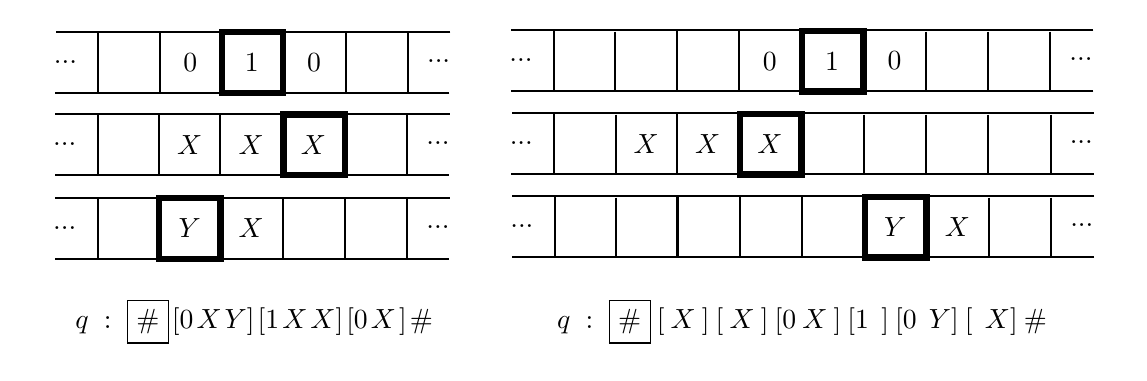
\begin{tikzpicture}[x=0.75pt,y=0.75pt,yscale=-1,xscale=1]
%uncomment if require: \path (0,446); %set diagram left start at 0, and has height of 446

%Straight Lines [id:da30015638181799353] 
\draw    (240.2,150.4) -- (109.4,150.4) -- (50.2,150.4) ;
%Straight Lines [id:da11411569986237446] 
\draw    (239.8,179.8) -- (50,179.8) ;
%Straight Lines [id:da29500831402425143] 
\draw    (70.6,150.6) -- (70.6,179.8) ;
%Straight Lines [id:da733451357781356] 
\draw    (100.2,151) -- (100.2,180.2) ;
%Straight Lines [id:da03010630232834921] 
\draw    (129.8,150.6) -- (129.8,179.8) ;
%Straight Lines [id:da445167041151461] 
\draw    (159.8,150.6) -- (159.8,179.8) ;
%Straight Lines [id:da2504444375488726] 
\draw    (189.8,150.6) -- (189.8,179.8) ;
%Straight Lines [id:da6446130969235513] 
\draw    (219.8,151) -- (219.8,180.2) ;
%Shape: Rectangle [id:dp7572905927556941] 
\draw  [line width=2.25]  (159.8,179.8) -- (130.2,179.8) -- (130.2,150.6) -- (159.8,150.6) -- cycle ;
%Straight Lines [id:da046077835472691175] 
\draw    (239.87,190.07) -- (109.07,190.07) -- (49.87,190.07) ;
%Straight Lines [id:da0944679329900775] 
\draw    (239.47,219.47) -- (49.67,219.47) ;
%Straight Lines [id:da8413340768410034] 
\draw    (70.27,190.27) -- (70.27,219.47) ;
%Straight Lines [id:da9817409758063647] 
\draw    (99.87,190.67) -- (99.87,219.87) ;
%Straight Lines [id:da97563264795794] 
\draw    (129.47,190.27) -- (129.47,219.47) ;
%Straight Lines [id:da4185457721864507] 
\draw    (159.47,190.27) -- (159.47,219.47) ;
%Straight Lines [id:da7023890172882994] 
\draw    (189.47,190.27) -- (189.47,219.47) ;
%Straight Lines [id:da9869975020440513] 
\draw    (219.47,190.67) -- (219.47,219.87) ;
%Shape: Rectangle [id:dp9890720482652489] 
\draw  [line width=2.25]  (189.47,219.47) -- (159.87,219.47) -- (159.87,190.27) -- (189.47,190.27) -- cycle ;
%Straight Lines [id:da5862728681013674] 
\draw    (239.87,230.4) -- (109.07,230.4) -- (49.87,230.4) ;
%Straight Lines [id:da6041220944668728] 
\draw    (239.47,259.8) -- (49.67,259.8) ;
%Straight Lines [id:da24766733675893904] 
\draw    (70.27,230.6) -- (70.27,259.8) ;
%Straight Lines [id:da5558397972695843] 
\draw    (99.87,231) -- (99.87,260.2) ;
%Straight Lines [id:da23035091712651168] 
\draw    (129.47,230.6) -- (129.47,259.8) ;
%Straight Lines [id:da49313971891750796] 
\draw    (159.47,230.6) -- (159.47,259.8) ;
%Straight Lines [id:da05108193021026186] 
\draw    (189.47,230.6) -- (189.47,259.8) ;
%Straight Lines [id:da39089490065153654] 
\draw    (219.47,231) -- (219.47,260.2) ;
%Shape: Rectangle [id:dp6582319445512015] 
\draw  [line width=2.25]  (129.47,259.8) -- (99.87,259.8) -- (99.87,230.6) -- (129.47,230.6) -- cycle ;
%Straight Lines [id:da1882557533312399] 
\draw    (550,149.73) -- (328.9,149.73) -- (269.7,149.73) ;
%Straight Lines [id:da5656120206785125] 
\draw    (550,179.13) -- (269.5,179.13) ;
%Straight Lines [id:da6013307837037323] 
\draw    (290.1,149.93) -- (290.1,179.13) ;
%Straight Lines [id:da2998129455294054] 
\draw    (319.7,150.33) -- (319.7,179.53) ;
%Straight Lines [id:da6202490683510069] 
\draw    (349.3,149.93) -- (349.3,179.13) ;
%Straight Lines [id:da12639843780905013] 
\draw    (379.3,149.93) -- (379.3,179.13) ;
%Straight Lines [id:da7315797833062889] 
\draw    (409.3,149.93) -- (409.3,179.13) ;
%Straight Lines [id:da7711503945631999] 
\draw    (439.3,150.33) -- (439.3,179.53) ;
%Shape: Rectangle [id:dp9547080445432563] 
\draw  [line width=2.25]  (439.3,179.13) -- (409.7,179.13) -- (409.7,149.93) -- (439.3,149.93) -- cycle ;
%Straight Lines [id:da5443274202623749] 
\draw    (469.3,150.33) -- (469.3,179.53) ;
%Straight Lines [id:da5364959360357715] 
\draw    (499.3,150.33) -- (499.3,179.53) ;
%Straight Lines [id:da36154191065050156] 
\draw    (529.3,150.33) -- (529.3,179.53) ;
%Straight Lines [id:da616132435625951] 
\draw    (550.15,189.73) -- (329.05,189.73) -- (269.85,189.73) ;
%Straight Lines [id:da79087562966597] 
\draw    (550.15,219.13) -- (269.65,219.13) ;
%Straight Lines [id:da9459536848119623] 
\draw    (290.25,189.93) -- (290.25,219.13) ;
%Straight Lines [id:da46782163143922295] 
\draw    (319.85,190.33) -- (319.85,219.53) ;
%Straight Lines [id:da7981948161257817] 
\draw    (349.45,189.93) -- (349.45,219.13) ;
%Straight Lines [id:da06855090432787092] 
\draw    (379.45,189.93) -- (379.45,219.13) ;
%Straight Lines [id:da20336495797736176] 
\draw    (409.45,189.93) -- (409.45,219.13) ;
%Straight Lines [id:da8523732422436843] 
\draw    (439.45,190.33) -- (439.45,219.53) ;
%Shape: Rectangle [id:dp07481634482569866] 
\draw  [line width=2.25]  (409.45,219.13) -- (379.85,219.13) -- (379.85,189.93) -- (409.45,189.93) -- cycle ;
%Straight Lines [id:da6380182999551376] 
\draw    (469.45,190.33) -- (469.45,219.53) ;
%Straight Lines [id:da23324877571651936] 
\draw    (499.45,190.33) -- (499.45,219.53) ;
%Straight Lines [id:da8976337300410169] 
\draw    (529.45,190.33) -- (529.45,219.53) ;
%Straight Lines [id:da061723972237821334] 
\draw    (550.4,229.73) -- (329.3,229.73) -- (270.1,229.73) ;
%Straight Lines [id:da34453572964027046] 
\draw    (550.4,259.13) -- (269.9,259.13) ;
%Straight Lines [id:da12561481810959085] 
\draw    (290.5,229.93) -- (290.5,259.13) ;
%Straight Lines [id:da1879532672587354] 
\draw    (320.1,230.33) -- (320.1,259.53) ;
%Straight Lines [id:da8026255207608686] 
\draw    (349.7,229.93) -- (349.7,259.13) ;
%Straight Lines [id:da3839979912893807] 
\draw    (379.7,229.93) -- (379.7,259.13) ;
%Straight Lines [id:da2671815060661715] 
\draw    (409.7,229.93) -- (409.7,259.13) ;
%Straight Lines [id:da4064867860363921] 
\draw    (439.7,230.33) -- (439.7,259.53) ;
%Shape: Rectangle [id:dp5125794035010658] 
\draw  [line width=2.25]  (469.7,259.13) -- (440.1,259.13) -- (440.1,229.93) -- (469.7,229.93) -- cycle ;
%Straight Lines [id:da2285589956250209] 
\draw    (469.7,230.33) -- (469.7,259.53) ;
%Straight Lines [id:da9042249167135066] 
\draw    (499.7,230.33) -- (499.7,259.53) ;
%Straight Lines [id:da4011962093886343] 
\draw    (529.7,230.33) -- (529.7,259.53) ;

% Text Node
\draw (85.4,165.2) node   [align=left] {\begin{minipage}[lt]{20.13pt}\setlength\topsep{0pt}
\begin{center}
\Vtextvisiblespace
\end{center}

\end{minipage}};
% Text Node
\draw (115,165.2) node   [align=left] {\begin{minipage}[lt]{20.13pt}\setlength\topsep{0pt}
\begin{center}
$0$
\end{center}

\end{minipage}};
% Text Node
\draw (144.6,165.2) node   [align=left] {\begin{minipage}[lt]{20.13pt}\setlength\topsep{0pt}
\begin{center}
$1$
\end{center}

\end{minipage}};
% Text Node
\draw (174.6,165.2) node   [align=left] {\begin{minipage}[lt]{20.13pt}\setlength\topsep{0pt}
\begin{center}
$0$
\end{center}

\end{minipage}};
% Text Node
\draw (204.6,165.2) node   [align=left] {\begin{minipage}[lt]{20.13pt}\setlength\topsep{0pt}
\begin{center}
\Vtextvisiblespace
\end{center}

\end{minipage}};
% Text Node
\draw (234.6,165.6) node   [align=left] {\begin{minipage}[lt]{20.13pt}\setlength\topsep{0pt}
\begin{center}
...
\end{center}

\end{minipage}};
% Text Node
\draw (54.8,166.2) node   [align=left] {\begin{minipage}[lt]{20.13pt}\setlength\topsep{0pt}
\begin{center}
...
\end{center}

\end{minipage}};
% Text Node
\draw (85.07,204.87) node   [align=left] {\begin{minipage}[lt]{20.13pt}\setlength\topsep{0pt}
\begin{center}
\Vtextvisiblespace
\end{center}

\end{minipage}};
% Text Node
\draw (114.67,204.87) node   [align=left] {\begin{minipage}[lt]{20.13pt}\setlength\topsep{0pt}
\begin{center}
$X$
\end{center}

\end{minipage}};
% Text Node
\draw (144.27,204.87) node   [align=left] {\begin{minipage}[lt]{20.13pt}\setlength\topsep{0pt}
\begin{center}
$X$
\end{center}

\end{minipage}};
% Text Node
\draw (174.27,204.87) node   [align=left] {\begin{minipage}[lt]{20.13pt}\setlength\topsep{0pt}
\begin{center}
$X$
\end{center}

\end{minipage}};
% Text Node
\draw (204.27,204.87) node   [align=left] {\begin{minipage}[lt]{20.13pt}\setlength\topsep{0pt}
\begin{center}
\Vtextvisiblespace
\end{center}

\end{minipage}};
% Text Node
\draw (234.27,205.27) node   [align=left] {\begin{minipage}[lt]{20.13pt}\setlength\topsep{0pt}
\begin{center}
...
\end{center}

\end{minipage}};
% Text Node
\draw (54.47,205.87) node   [align=left] {\begin{minipage}[lt]{20.13pt}\setlength\topsep{0pt}
\begin{center}
...
\end{center}

\end{minipage}};
% Text Node
\draw (85.07,245.2) node   [align=left] {\begin{minipage}[lt]{20.13pt}\setlength\topsep{0pt}
\begin{center}
\Vtextvisiblespace
\end{center}

\end{minipage}};
% Text Node
\draw (114.67,245.2) node   [align=left] {\begin{minipage}[lt]{20.13pt}\setlength\topsep{0pt}
\begin{center}
$Y$
\end{center}

\end{minipage}};
% Text Node
\draw (144.27,245.2) node   [align=left] {\begin{minipage}[lt]{20.13pt}\setlength\topsep{0pt}
\begin{center}
$X$
\end{center}

\end{minipage}};
% Text Node
\draw (174.27,245.2) node   [align=left] {\begin{minipage}[lt]{20.13pt}\setlength\topsep{0pt}
\begin{center}
\Vtextvisiblespace
\end{center}

\end{minipage}};
% Text Node
\draw (204.27,245.2) node   [align=left] {\begin{minipage}[lt]{20.13pt}\setlength\topsep{0pt}
\begin{center}
\Vtextvisiblespace
\end{center}

\end{minipage}};
% Text Node
\draw (234.27,245.6) node   [align=left] {\begin{minipage}[lt]{20.13pt}\setlength\topsep{0pt}
\begin{center}
...
\end{center}

\end{minipage}};
% Text Node
\draw (54.47,246.2) node   [align=left] {\begin{minipage}[lt]{20.13pt}\setlength\topsep{0pt}
\begin{center}
...
\end{center}

\end{minipage}};
% Text Node
\draw (304.9,164.53) node   [align=left] {\begin{minipage}[lt]{20.13pt}\setlength\topsep{0pt}
\begin{center}
\Vtextvisiblespace
\end{center}

\end{minipage}};
% Text Node
\draw (334.5,164.53) node   [align=left] {\begin{minipage}[lt]{20.13pt}\setlength\topsep{0pt}
\begin{center}
\Vtextvisiblespace
\end{center}

\end{minipage}};
% Text Node
\draw (364.1,164.53) node   [align=left] {\begin{minipage}[lt]{20.13pt}\setlength\topsep{0pt}
\begin{center}
\Vtextvisiblespace
\end{center}

\end{minipage}};
% Text Node
\draw (394.1,164.53) node   [align=left] {\begin{minipage}[lt]{20.13pt}\setlength\topsep{0pt}
\begin{center}
$0$
\end{center}

\end{minipage}};
% Text Node
\draw (424.1,164.53) node   [align=left] {\begin{minipage}[lt]{20.13pt}\setlength\topsep{0pt}
\begin{center}
$1$
\end{center}

\end{minipage}};
% Text Node
\draw (274.3,165.53) node   [align=left] {\begin{minipage}[lt]{20.13pt}\setlength\topsep{0pt}
\begin{center}
...
\end{center}

\end{minipage}};
% Text Node
\draw (454.25,164.33) node   [align=left] {\begin{minipage}[lt]{20.13pt}\setlength\topsep{0pt}
\begin{center}
$0$
\end{center}

\end{minipage}};
% Text Node
\draw (484.1,164.53) node   [align=left] {\begin{minipage}[lt]{20.13pt}\setlength\topsep{0pt}
\begin{center}
\Vtextvisiblespace
\end{center}

\end{minipage}};
% Text Node
\draw (514.1,164.53) node   [align=left] {\begin{minipage}[lt]{20.13pt}\setlength\topsep{0pt}
\begin{center}
\Vtextvisiblespace
\end{center}

\end{minipage}};
% Text Node
\draw (544.1,164.93) node   [align=left] {\begin{minipage}[lt]{20.13pt}\setlength\topsep{0pt}
\begin{center}
...
\end{center}

\end{minipage}};
% Text Node
\draw (305.05,204.53) node   [align=left] {\begin{minipage}[lt]{20.13pt}\setlength\topsep{0pt}
\begin{center}
\Vtextvisiblespace
\end{center}

\end{minipage}};
% Text Node
\draw (334.65,204.53) node   [align=left] {\begin{minipage}[lt]{20.13pt}\setlength\topsep{0pt}
\begin{center}
$X$
\end{center}

\end{minipage}};
% Text Node
\draw (364.25,204.53) node   [align=left] {\begin{minipage}[lt]{20.13pt}\setlength\topsep{0pt}
\begin{center}
$X$
\end{center}

\end{minipage}};
% Text Node
\draw (394.25,204.53) node   [align=left] {\begin{minipage}[lt]{20.13pt}\setlength\topsep{0pt}
\begin{center}
$X$
\end{center}

\end{minipage}};
% Text Node
\draw (424.25,204.53) node   [align=left] {\begin{minipage}[lt]{20.13pt}\setlength\topsep{0pt}
\begin{center}
\Vtextvisiblespace
\end{center}

\end{minipage}};
% Text Node
\draw (274.45,205.53) node   [align=left] {\begin{minipage}[lt]{20.13pt}\setlength\topsep{0pt}
\begin{center}
...
\end{center}

\end{minipage}};
% Text Node
\draw (454.4,204.33) node   [align=left] {\begin{minipage}[lt]{20.13pt}\setlength\topsep{0pt}
\begin{center}
\Vtextvisiblespace
\end{center}

\end{minipage}};
% Text Node
\draw (484.25,204.53) node   [align=left] {\begin{minipage}[lt]{20.13pt}\setlength\topsep{0pt}
\begin{center}
\Vtextvisiblespace
\end{center}

\end{minipage}};
% Text Node
\draw (514.25,204.53) node   [align=left] {\begin{minipage}[lt]{20.13pt}\setlength\topsep{0pt}
\begin{center}
\Vtextvisiblespace
\end{center}

\end{minipage}};
% Text Node
\draw (544.25,204.93) node   [align=left] {\begin{minipage}[lt]{20.13pt}\setlength\topsep{0pt}
\begin{center}
...
\end{center}

\end{minipage}};
% Text Node
\draw (305.3,244.53) node   [align=left] {\begin{minipage}[lt]{20.13pt}\setlength\topsep{0pt}
\begin{center}
\Vtextvisiblespace
\end{center}

\end{minipage}};
% Text Node
\draw (334.9,244.53) node   [align=left] {\begin{minipage}[lt]{20.13pt}\setlength\topsep{0pt}
\begin{center}
\Vtextvisiblespace
\end{center}

\end{minipage}};
% Text Node
\draw (364.5,244.53) node   [align=left] {\begin{minipage}[lt]{20.13pt}\setlength\topsep{0pt}
\begin{center}
\Vtextvisiblespace
\end{center}

\end{minipage}};
% Text Node
\draw (394.5,244.53) node   [align=left] {\begin{minipage}[lt]{20.13pt}\setlength\topsep{0pt}
\begin{center}
\Vtextvisiblespace
\end{center}

\end{minipage}};
% Text Node
\draw (424.5,244.53) node   [align=left] {\begin{minipage}[lt]{20.13pt}\setlength\topsep{0pt}
\begin{center}
\Vtextvisiblespace
\end{center}

\end{minipage}};
% Text Node
\draw (274.7,245.53) node   [align=left] {\begin{minipage}[lt]{20.13pt}\setlength\topsep{0pt}
\begin{center}
...
\end{center}

\end{minipage}};
% Text Node
\draw (454.65,244.33) node   [align=left] {\begin{minipage}[lt]{20.13pt}\setlength\topsep{0pt}
\begin{center}
$Y$
\end{center}

\end{minipage}};
% Text Node
\draw (484.5,244.53) node   [align=left] {\begin{minipage}[lt]{20.13pt}\setlength\topsep{0pt}
\begin{center}
$X$
\end{center}

\end{minipage}};
% Text Node
\draw (514.5,244.53) node   [align=left] {\begin{minipage}[lt]{20.13pt}\setlength\topsep{0pt}
\begin{center}
\Vtextvisiblespace
\end{center}

\end{minipage}};
% Text Node
\draw (544.5,244.93) node   [align=left] {\begin{minipage}[lt]{20.13pt}\setlength\topsep{0pt}
\begin{center}
...
\end{center}

\end{minipage}};
% Text Node
\draw (145.67,282.4) node   [align=left] {\begin{minipage}[lt]{129.2pt}\setlength\topsep{0pt}
\begin{center}
$$q\;:\;\fbox{\#}\:[0\:X\:\cabezal{Y}]\:[\cabezal{1}\:X\:X]\:[0\:\cabezal{X}\:\Vtextvisiblespace]\:\#$$
\end{center}

\end{minipage}};
% Text Node
\draw (409.67,282.4) node   [align=left] {\begin{minipage}[lt]{190.85pt}\setlength\topsep{0pt}
\begin{center}
$$q\;:\;\fbox{\#}\:[\Vtextvisiblespace\:X\:\Vtextvisiblespace]\:[\Vtextvisiblespace\:X\:\Vtextvisiblespace]\:[0\:\cabezal{X}\:\Vtextvisiblespace]\:[\cabezal{1}\:\Vtextvisiblespace\:\Vtextvisiblespace]\:[0\:\Vtextvisiblespace\:\cabezal{Y}]\:[\Vtextvisiblespace\:\Vtextvisiblespace\:X]\:\#$$
\end{center}

\end{minipage}};


\end{tikzpicture}
\caption{Dos configuraciones de $\widetilde{M}$ para una configuración de $M$}
\label{fig:configuraciones-mtilde}
\end{figure}
% ===================+

Observemos que varias configuraciones de $\widetilde{M}$ son posibles, dado que las $k$ cintas son independientes (no importa cómo las ``apilamos'', y esto no tiene efecto en el proceso de cálculo). Esta característica de nuestra codificación se evidencia en la \cref{fig:configuraciones-mtilde}. Sin embargo, esta independencia hace que esta peculiaridad no nos afecte: simplemente dejamos que la máquina vaya computando y vamos aplicando las transiciones y modificando las transiciones según se dicte.

Describir de forma exacta el conjunto de estados $\widetilde{Q}$ y la función de transición $\widetilde{\delta}$ es un proceso arduo, que se detalla en el \cref{ap:demostraciones-adicionales} (véase la \cref{prop:ap-mtm}). En esta demostración, nos limitaremos a explicar su comportamiento.

La máquina comienza con la configuración inicial para la entrada: $u=u_1\:u_2\:...\:u_n\in A^*$:
$$
    q_0\;:\;\fbox{\#}\:[\widecheck{u_1}\:\underbrace{\widecheck{\Vtextvisiblespace} \:... \:\widecheck{\Vtextvisiblespace}}_{k-1)}]\:[u_2\:\underbrace{{\Vtextvisiblespace} \:... \:{\Vtextvisiblespace}}_{k-1)}]\:...\:[u_n\:\underbrace{{\Vtextvisiblespace} \:... \:{\Vtextvisiblespace}}_{k-1)}]\:\#
$$
A continuación, va aplicando los movimientos de $\delta$ cinta a cinta y cabezal a cabezal. Llamaremos a estas cintas y cabezales ``cintas virtuales'' y ``cabezales virtuales'', respectivamente.

Para ello, comienza escaneando toda la cinta desde el delimitador $\#$ izquierdo, y almacena los valores de los cabezales virtuales en estados de $\widetilde{Q}$. El conjunto $\widetilde{Q}$ es ampliado para poder efectuar esta acción de ``memorización''. A continuación, volvemos al principio de la cinta, y vamos efectuando cada una de las acciones de $M$, por cada cinta virtual. Si en algún momento, al desplazar cada cabezal virtual nos lo coloca sobre un delimitador $\#$, reemplazamos la posición de la cinta por el símbolo blanco de $\widetilde{M}$, $[\Vtextvisiblespace^k]$, y desplazamos $\#$ a la izquierda o derecha según sea necesario.

Una vez hecho esto, cambiamos el estado inicial por el estado correspondiente según $\delta$ y así sucesivamente. El conjunto $F$ es el mismo dado que vamos pasando por los mismos estados de $Q$ en $\widetilde{Q}$.

Es fácil ver que $L(M)=L(\widetilde{M})$, dado que hemos creado una máquina que imita a la perfección el proceso de cálculo de $M$, y en caso de parar, para en un estado de $Q$. Las palabras aceptadas serán aquellas en las que, una vez que la máquina haya parado, el estado esté en $F$.
\end{proofw}

Pensemos un momento en las consecuencias de que estos dos modelos de cálculo sean equivalentes. En primer lugar, nos da una idea del alcance de la máquina de Turing monocinta: introduciendo más complejidad en su descripción, no podemos aspirar a crear algoritmos más complejos, pues siempre podremos encontrar un algoritmo equivalente en una máquina de una sola cinta. Esto, como comentábamos al comienzo del capítulo, nos da una pista de una de las tesis más relevantes de las ciencias de la computación en la actualidad, y que discutimos en la \cref{sec:church-turing}.

En segundo lugar, esto nos da una ventaja a la hora de querer resolver problemas: poder describir un programa en un modelo que nos da una mayor flexibilidad es mucho más sencillo.

Al avanzar en esta sección, es importante mantener en mente estas dos observaciones. Ahora, introduciremos un nuevo modelo computacional: la máquina de acceso aleatorio. \cite{MacCormick2018}
% ===================+


% ===================+
\begin{definicion}[Máquina de Turing de acceso aleatorio]
\index{máquina de acceso aleatorio}
Una \emph{máquina de Turing de acceso aleatorio}\index{máquina de Turing!de acceso aleatorio} con $k$ cintas es una máquina de Turing multicinta de $k$ cintas con dos cintas adicionales, limitadas a la izquierda:
\begin{itemize}
    \item Una \textit{cinta de dirección}\index{cinta!de dirección}, que almacena un número natural $n\in\mathbb{N}$.\footnote{Suponemos $0\notin\mathbb{N}$.}
    \item Una cinta llamada \textit{RAM}\index{RAM}, que almacena símbolos en cada una de sus pistas.
\end{itemize}
Denotamos como $\text{RAM}[n]$ a la $n$-ésima pista de la RAM.

La función $\delta : Q \times \mathbb{N} \times B \times B^k \longrightarrow \left(Q \times \mathbb{N} \times B \times (B \times \{I, D, S\})^k\right) \cup \emptyset$ será de la forma:
$$
\delta(q, b_1, b_2, ..., b_k) = \emptyset
$$
para las transiciones no definidas, y para las definidas:
\begin{multline}
    \delta(q, n, r, b_1, b_2, ..., b_k) = (p, m, s, c_1, M_1, c_2, M_2, ..., c_k, M_k),\\ \text{ con }q,p\in Q, n, m, \in \mathbb{N}, r, s, b_i, c_i \in B, M_i \in \{I, D, S\},\;\forall i \in \{1, 2, ..., k\}
\end{multline}
La transición definida se ejecutará si el valor de $\text{RAM}[n]=r$, y tras ejecutarla el valor de $\text{RAM}[n]$ cambiará a $s$, y el valor de la cinta de dirección cambiará de $n$ a $m$. Es decir, en una única transición, es capaz de acceder a la posición de la RAM, modificarla, y cambiar la posición de la RAM.

Una configuración\index{configuración!de una máquina de Turing de acceso aleatorio} de la máquina se especificará mediante:
$$q\;:\;r\:;\:w_1\:,\:w_2\:,\:...\:,\:w_k$$
con un símbolo de cada cinta $w_1, w_2, ..., w_k$ debidamente recuadrado, y con un símbolo de $r$ recuadrado, concretamente, aquel al que apunte la cinta de dirección.
\end{definicion}
% ===================+

Podemos ver un ejemplo de tal configuración en la \cref{fig:maquina-turing-aleatorio}.

Probar que una máquina de Turing de acceso aleatorio puede ser simulada mediante una máquina de Turing multicinta es sencillo pero tedioso. En la \cref{prop:multicinta-a-aleatorio} se explican las rutinas que serían necesarias para tal simulación.

% ===================+
\begin{proposicion}\label{prop:multicinta-a-aleatorio}
Toda máquina de Turing de acceso aleatorio de $k$ puede ser simulada por una máquina de Turing multicinta.
\end{proposicion}
\begin{proof}
Para probar esto, necesitaremos una máquina de Turing de $k+2$ cintas. Las dos últimas cintas serán la cinta de dirección ($k+1$-ésima cinta) y la RAM ($k+2$-ésima cinta). A continuación, vemos que:

\begin{itemize}
    \item[(1)] Podemos crear una rutina que reemplace el símbolo de la posición del cabezal en la cinta $k+2$ por otro.
    \item[(2)] Podemos crear una rutina que modifique la dirección de la cinta $k+1$.
    \item[(3)] Podemos crear una rutina que, dada una dirección en la cinta $k+1$, mueva el cabezal de la cinta $k+2$ a la posición correspondiente. Podríamos implementar una rutina que vaya contando hasta el número de la cinta $k+1$ y, cada vez que va contando, va moviendo el cabezal de la cinta $k+2$ una posición a la derecha, comenzando al principio.
\end{itemize}
Implementar la operación adicional atómica de la máquina de Turing de acceso aleatorio en esta máquina multicinta es sencillo: podemos acceder al valor de $\text{RAM}[n]$, $r$, viendo dónde se encuentra el cabezal en la cinta $k+2$. En función de esto, ejecutamos la transición necesaria. Tras esto, modificamos $\text{RAM}[n]$ a $s$ ejecutando la rutina (1), y cambiamos la dirección de la cinta $k+1$ ejecutando (2). Finalmente, modificamos la posición del cabezal en la cinta $k+2$ ejecutando la rutina (3). 
\end{proof}
% ===================+

% ===================+
\begin{figure}[H]
\centering
$$q_3\;:\;1\:a\:b\:\fbox{$2$}\:;\:2\:\fbox{$X$}\:X\:,\:\fbox{$1$}\:0\:,\:...\:,\:w_k$$
\tikzset{every picture/.style={line width=0.75pt}} %set default line width to 0.75pt        

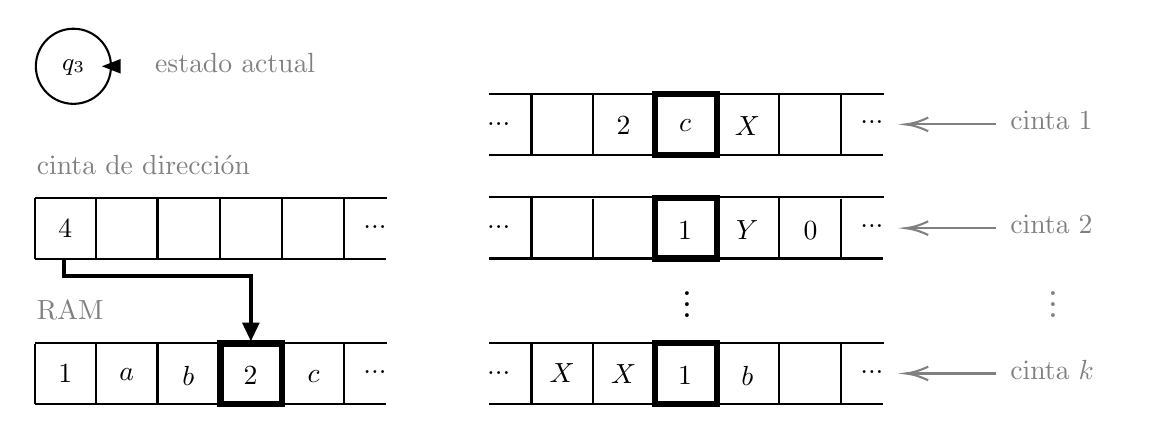
\begin{tikzpicture}[x=0.75pt,y=0.75pt,yscale=-1,xscale=1]
%uncomment if require: \path (0,446); %set diagram left start at 0, and has height of 446

%Shape: Triangle [id:dp22833396870153844] 
\draw  [fill={rgb, 255:red, 0; green, 0; blue, 0 }  ,fill opacity=1 ] (134.4,87) -- (141.6,84.2) -- (141.6,89.8) -- cycle ;
%Straight Lines [id:da9502918156750955] 
\draw    (270.2,150.4) -- (139.4,150.4) -- (100.6,150.4) ;
%Straight Lines [id:da2435786607255459] 
\draw    (269.8,179.8) -- (100.6,179.8) ;
%Straight Lines [id:da14005386027485822] 
\draw    (100.6,150.6) -- (100.6,179.8) ;
%Straight Lines [id:da3540718886756644] 
\draw    (130.2,151) -- (130.2,180.2) ;
%Straight Lines [id:da4139388876669716] 
\draw    (159.8,150.6) -- (159.8,179.8) ;
%Straight Lines [id:da5218209879340381] 
\draw    (189.8,150.6) -- (189.8,179.8) ;
%Straight Lines [id:da7791625461953589] 
\draw    (219.8,150.6) -- (219.8,179.8) ;
%Straight Lines [id:da7244728783081309] 
\draw    (249.8,151) -- (249.8,180.2) ;
%Shape: Rectangle [id:dp37161496605875444] 
%Straight Lines [id:da46389211227924587] 
\draw    (509.6,220.2) -- (378.8,220.2) -- (319.6,220.2) ;
%Straight Lines [id:da031153687975910227] 
\draw    (509.2,249.6) -- (319.4,249.6) ;
%Straight Lines [id:da930892660964344] 
\draw    (340,220.4) -- (340,249.6) ;
%Straight Lines [id:da8359375296699874] 
\draw    (369.6,220.8) -- (369.6,250) ;
%Straight Lines [id:da9248713052561113] 
\draw    (399.2,220.4) -- (399.2,249.6) ;
%Straight Lines [id:da9565266138427906] 
\draw    (429.2,220.4) -- (429.2,249.6) ;
%Straight Lines [id:da6204065712086833] 
\draw    (459.2,220.4) -- (459.2,249.6) ;
%Straight Lines [id:da8115307864724526] 
\draw    (489.2,220.8) -- (489.2,250) ;
%Shape: Rectangle [id:dp9651839314118411] 
\draw  [line width=2.25]  (429.2,249.6) -- (399.6,249.6) -- (399.6,220.4) -- (429.2,220.4) -- cycle ;
%Straight Lines [id:da49928112407779013] 
\draw [color={rgb, 255:red, 128; green, 128; blue, 128 }  ,draw opacity=1 ]   (563.8,235) -- (522.2,235) ;
\draw [shift={(520.2,235)}, rotate = 360] [color={rgb, 255:red, 128; green, 128; blue, 128 }  ,draw opacity=1 ][line width=0.75]    (10.93,-3.29) .. controls (6.95,-1.4) and (3.31,-0.3) .. (0,0) .. controls (3.31,0.3) and (6.95,1.4) .. (10.93,3.29)   ;
%Shape: Circle [id:dp4875732591382371] 
\draw   (101.2,87) .. controls (101.2,77) and (109.31,68.9) .. (119.3,68.9) .. controls (129.3,68.9) and (137.4,77) .. (137.4,87) .. controls (137.4,97) and (129.3,105.1) .. (119.3,105.1) .. controls (109.31,105.1) and (101.2,97) .. (101.2,87) -- cycle ;
%Straight Lines [id:da4059064140058737] 
\draw    (270.2,220.4) -- (139.4,220.4) -- (100.6,220.4) ;
%Straight Lines [id:da903225832956271] 
\draw    (269.8,249.8) -- (100.6,249.8) ;
%Straight Lines [id:da8283523716346759] 
\draw    (100.6,220.6) -- (100.6,249.8) ;
%Straight Lines [id:da45368269415437656] 
\draw    (130.2,221) -- (130.2,250.2) ;
%Straight Lines [id:da9876183704449528] 
\draw    (159.8,220.6) -- (159.8,249.8) ;
%Straight Lines [id:da7481690903519229] 
\draw    (189.8,220.6) -- (189.8,249.8) ;
%Straight Lines [id:da3667149686910236] 
\draw    (219.8,220.6) -- (219.8,249.8) ;
%Straight Lines [id:da41652912310539403] 
\draw    (249.8,221) -- (249.8,250.2) ;
%Shape: Rectangle [id:dp2939622979641314] 
\draw  [line width=2.25]  (219.8,249.8) -- (190.2,249.8) -- (190.2,220.6) -- (219.8,220.6) -- cycle ;
%Straight Lines [id:da17099329842973332] 
\draw    (509.6,150.2) -- (378.8,150.2) -- (319.6,150.2) ;
%Straight Lines [id:da7653261528594799] 
\draw    (509.2,179.6) -- (319.4,179.6) ;
%Straight Lines [id:da8224438701900565] 
\draw    (340,150.4) -- (340,179.6) ;
%Straight Lines [id:da0390014763030202] 
\draw    (369.6,150.8) -- (369.6,180) ;
%Straight Lines [id:da07167765925752012] 
\draw    (399.2,150.4) -- (399.2,179.6) ;
%Straight Lines [id:da6912566029119143] 
\draw    (429.2,150.4) -- (429.2,179.6) ;
%Straight Lines [id:da15621954450232556] 
\draw    (459.2,150.4) -- (459.2,179.6) ;
%Straight Lines [id:da6118022257422364] 
\draw    (489.2,150.8) -- (489.2,180) ;
%Shape: Rectangle [id:dp1527357830072993] 
\draw  [line width=2.25]  (429.2,179.6) -- (399.6,179.6) -- (399.6,150.4) -- (429.2,150.4) -- cycle ;
%Straight Lines [id:da29868173223912486] 
\draw [color={rgb, 255:red, 128; green, 128; blue, 128 }  ,draw opacity=1 ]   (563.8,165) -- (522.2,165) ;
\draw [shift={(520.2,165)}, rotate = 360] [color={rgb, 255:red, 128; green, 128; blue, 128 }  ,draw opacity=1 ][line width=0.75]    (10.93,-3.29) .. controls (6.95,-1.4) and (3.31,-0.3) .. (0,0) .. controls (3.31,0.3) and (6.95,1.4) .. (10.93,3.29)   ;
%Straight Lines [id:da045321875173484516] 
\draw    (509.6,100.2) -- (378.8,100.2) -- (319.6,100.2) ;
%Straight Lines [id:da8155961414859514] 
\draw    (509.2,129.6) -- (319.4,129.6) ;
%Straight Lines [id:da23342429127843967] 
\draw    (340,100.4) -- (340,129.6) ;
%Straight Lines [id:da31120915926348136] 
\draw    (369.6,100.8) -- (369.6,130) ;
%Straight Lines [id:da33862890436022686] 
\draw    (399.2,100.4) -- (399.2,129.6) ;
%Straight Lines [id:da7874244230618799] 
\draw    (429.2,100.4) -- (429.2,129.6) ;
%Straight Lines [id:da09908575120999275] 
\draw    (459.2,100.4) -- (459.2,129.6) ;
%Straight Lines [id:da0946836215231126] 
\draw    (489.2,100.8) -- (489.2,130) ;
%Shape: Rectangle [id:dp5474970998625763] 
\draw  [line width=2.25]  (429.2,129.6) -- (399.6,129.6) -- (399.6,100.4) -- (429.2,100.4) -- cycle ;
%Straight Lines [id:da9655890926468969] 
\draw [color={rgb, 255:red, 128; green, 128; blue, 128 }  ,draw opacity=1 ]   (563.8,115) -- (522.2,115) ;
\draw [shift={(520.2,115)}, rotate = 360] [color={rgb, 255:red, 128; green, 128; blue, 128 }  ,draw opacity=1 ][line width=0.75]    (10.93,-3.29) .. controls (6.95,-1.4) and (3.31,-0.3) .. (0,0) .. controls (3.31,0.3) and (6.95,1.4) .. (10.93,3.29)   ;
%Straight Lines [id:da20988241940575603] 
\draw    (204.8,202.2) -- (204.8,216.4) ;
\draw [shift={(204.8,219.4)}, rotate = 270] [fill={rgb, 255:red, 0; green, 0; blue, 0 }  ][line width=0.08]  [draw opacity=0] (8.93,-4.29) -- (0,0) -- (8.93,4.29) -- cycle    ;
%Shape: Right Angle [id:dp6173925874176376] 
\draw  [line width=1.5]  (181.4,188.2) -- (114.6,188.2) -- (114.6,179.8) ;
%Shape: Right Angle [id:dp4259446592719347] 
\draw  [line width=1.5]  (159,188.2) -- (204.8,188.2) -- (204.8,213.8) ;

% Text Node
\draw (115.4,165.2) node   [align=left] {\begin{minipage}[lt]{20.13pt}\setlength\topsep{0pt}
\begin{center}
$4$
\end{center}

\end{minipage}};
% Text Node
\draw (145,165.6) node   [align=left] {\begin{minipage}[lt]{20.13pt}\setlength\topsep{0pt}
\begin{center}
\Vtextvisiblespace
\end{center}

\end{minipage}};
% Text Node
\draw (174.6,166.2) node   [align=left] {\begin{minipage}[lt]{20.13pt}\setlength\topsep{0pt}
\begin{center}
\Vtextvisiblespace
\end{center}

\end{minipage}};
% Text Node
\draw (204.6,166.2) node   [align=left] {\begin{minipage}[lt]{20.13pt}\setlength\topsep{0pt}
\begin{center}
\Vtextvisiblespace
\end{center}

\end{minipage}};
% Text Node
\draw (235,166.6) node   [align=left] {\begin{minipage}[lt]{20.13pt}\setlength\topsep{0pt}
\begin{center}
\Vtextvisiblespace
\end{center}

\end{minipage}};
% Text Node
\draw (264.6,165.6) node   [align=left] {\begin{minipage}[lt]{20.13pt}\setlength\topsep{0pt}
\begin{center}
...
\end{center}

\end{minipage}};
% Text Node
\draw (174.6,134.6) node  [color={rgb, 255:red, 128; green, 128; blue, 128 }  ,opacity=1 ] [align=left] {\begin{minipage}[lt]{109.34pt}\setlength\topsep{0pt}
cinta de dirección
\end{minipage}};
% Text Node
\draw (354.8,235) node   [align=left] {\begin{minipage}[lt]{20.13pt}\setlength\topsep{0pt}
\begin{center}
$X$
\end{center}

\end{minipage}};
% Text Node
\draw (384.4,235.4) node   [align=left] {\begin{minipage}[lt]{20.13pt}\setlength\topsep{0pt}
\begin{center}
$X$
\end{center}

\end{minipage}};
% Text Node
\draw (414,236) node   [align=left] {\begin{minipage}[lt]{20.13pt}\setlength\topsep{0pt}
\begin{center}
$1$
\end{center}

\end{minipage}};
% Text Node
\draw (444,236) node   [align=left] {\begin{minipage}[lt]{20.13pt}\setlength\topsep{0pt}
\begin{center}
$b$
\end{center}

\end{minipage}};
% Text Node
\draw (474.4,236.4) node   [align=left] {\begin{minipage}[lt]{20.13pt}\setlength\topsep{0pt}
\begin{center}
\Vtextvisiblespace
\end{center}

\end{minipage}};
% Text Node
\draw (504,235.4) node   [align=left] {\begin{minipage}[lt]{20.13pt}\setlength\topsep{0pt}
\begin{center}
...
\end{center}

\end{minipage}};
% Text Node
\draw (324.2,236) node   [align=left] {\begin{minipage}[lt]{20.13pt}\setlength\topsep{0pt}
\begin{center}
...
\end{center}

\end{minipage}};
% Text Node
\draw (414.9,197.6) node  [font=\Large] [align=left] {\begin{minipage}[lt]{129.61pt}\setlength\topsep{0pt}
\begin{center}
$\vdots$
\end{center}

\end{minipage}};
% Text Node
\draw (569.2,227.2) node [anchor=north west][inner sep=0.75pt]  [color={rgb, 255:red, 128; green, 128; blue, 128 }  ,opacity=1 ] [align=left] {cinta $k$};
% Text Node
\draw (591.33,197.6) node  [font=\Large,color={rgb, 255:red, 128; green, 128; blue, 128 }  ,opacity=1 ] [align=left] {\begin{minipage}[lt]{47.6pt}\setlength\topsep{0pt}
\begin{center}
$\vdots$
\end{center}

\end{minipage}};
% Text Node
\draw (213.5,85.4) node  [color={rgb, 255:red, 128; green, 128; blue, 128 }  ,opacity=1 ] [align=left] {\begin{minipage}[lt]{82.28pt}\setlength\topsep{0pt}
estado actual
\end{minipage}};
% Text Node
\draw (112.4,82.2) node [anchor=north west][inner sep=0.75pt]  [font=\small] [align=left] {$q_3$};
% Text Node
\draw (115.4,235.2) node   [align=left] {\begin{minipage}[lt]{20.13pt}\setlength\topsep{0pt}
\begin{center}
$1$
\end{center}

\end{minipage}};
% Text Node
\draw (145,235.6) node   [align=left] {\begin{minipage}[lt]{20.13pt}\setlength\topsep{0pt}
\begin{center}
$a$
\end{center}

\end{minipage}};
% Text Node
\draw (174.6,236.2) node   [align=left] {\begin{minipage}[lt]{20.13pt}\setlength\topsep{0pt}
\begin{center}
$b$
\end{center}

\end{minipage}};
% Text Node
\draw (204.6,236.2) node   [align=left] {\begin{minipage}[lt]{20.13pt}\setlength\topsep{0pt}
\begin{center}
$2$
\end{center}

\end{minipage}};
% Text Node
\draw (235,236.6) node   [align=left] {\begin{minipage}[lt]{20.13pt}\setlength\topsep{0pt}
\begin{center}
$c$
\end{center}

\end{minipage}};
% Text Node
\draw (264.6,235.6) node   [align=left] {\begin{minipage}[lt]{20.13pt}\setlength\topsep{0pt}
\begin{center}
...
\end{center}

\end{minipage}};
% Text Node
\draw (174.6,204.6) node  [color={rgb, 255:red, 128; green, 128; blue, 128 }  ,opacity=1 ] [align=left] {\begin{minipage}[lt]{109.34pt}\setlength\topsep{0pt}
RAM
\end{minipage}};
% Text Node
\draw (354.8,165) node   [align=left] {\begin{minipage}[lt]{20.13pt}\setlength\topsep{0pt}
\begin{center}
\Vtextvisiblespace
\end{center}

\end{minipage}};
% Text Node
\draw (384.4,165.4) node   [align=left] {\begin{minipage}[lt]{20.13pt}\setlength\topsep{0pt}
\begin{center}
\Vtextvisiblespace
\end{center}

\end{minipage}};
% Text Node
\draw (414,166) node   [align=left] {\begin{minipage}[lt]{20.13pt}\setlength\topsep{0pt}
\begin{center}
$1$
\end{center}

\end{minipage}};
% Text Node
\draw (444,166) node   [align=left] {\begin{minipage}[lt]{20.13pt}\setlength\topsep{0pt}
\begin{center}
$Y$
\end{center}

\end{minipage}};
% Text Node
\draw (474.4,166.4) node   [align=left] {\begin{minipage}[lt]{20.13pt}\setlength\topsep{0pt}
\begin{center}
$0$
\end{center}

\end{minipage}};
% Text Node
\draw (504,165.4) node   [align=left] {\begin{minipage}[lt]{20.13pt}\setlength\topsep{0pt}
\begin{center}
...
\end{center}

\end{minipage}};
% Text Node
\draw (324.2,166) node   [align=left] {\begin{minipage}[lt]{20.13pt}\setlength\topsep{0pt}
\begin{center}
...
\end{center}

\end{minipage}};
% Text Node
\draw (569.2,157.2) node [anchor=north west][inner sep=0.75pt]  [color={rgb, 255:red, 128; green, 128; blue, 128 }  ,opacity=1 ] [align=left] {cinta $2$};
% Text Node
\draw (354.8,115) node   [align=left] {\begin{minipage}[lt]{20.13pt}\setlength\topsep{0pt}
\begin{center}
\Vtextvisiblespace
\end{center}

\end{minipage}};
% Text Node
\draw (384.4,115.4) node   [align=left] {\begin{minipage}[lt]{20.13pt}\setlength\topsep{0pt}
\begin{center}
$2$
\end{center}

\end{minipage}};
% Text Node
\draw (414,116) node   [align=left] {\begin{minipage}[lt]{20.13pt}\setlength\topsep{0pt}
\begin{center}
$c$
\end{center}

\end{minipage}};
% Text Node
\draw (444,116) node   [align=left] {\begin{minipage}[lt]{20.13pt}\setlength\topsep{0pt}
\begin{center}
$X$
\end{center}

\end{minipage}};
% Text Node
\draw (474.4,116.4) node   [align=left] {\begin{minipage}[lt]{20.13pt}\setlength\topsep{0pt}
\begin{center}
\Vtextvisiblespace
\end{center}

\end{minipage}};
% Text Node
\draw (504,115.4) node   [align=left] {\begin{minipage}[lt]{20.13pt}\setlength\topsep{0pt}
\begin{center}
...
\end{center}

\end{minipage}};
% Text Node
\draw (324.2,116) node   [align=left] {\begin{minipage}[lt]{20.13pt}\setlength\topsep{0pt}
\begin{center}
...
\end{center}

\end{minipage}};
% Text Node
\draw (569.2,107.2) node [anchor=north west][inner sep=0.75pt]  [color={rgb, 255:red, 128; green, 128; blue, 128 }  ,opacity=1 ] [align=left] {cinta $1$};


\end{tikzpicture}
\caption{Máquina de Turing de acceso aleatorio}
\label{fig:maquina-turing-aleatorio}
\end{figure}
% ===================+

A continuación, continuaremos con la cadena de simulaciones. Para ello, introduciremos una definición de \emph{ordenador}. Ésta es una simplificación de la arquitectura de un ordenador pero, a efectos prácticos, todos los ordenadores modernos siguen la estructura que se especifica en la \cref{def:ordenador}. \cite{Nisan2005}

% ===================+
\begin{definicion}[Ordenador moderno]\label{def:ordenador}
Definimos un \emph{ordenador moderno}\index{ordenador moderno} como aquel que dispone de los siguientes elementos:
\begin{itemize}
    \item \textbf{Registros.}\index{registro} Un registro permite almacenar exactamente una unidad de información, en binario. Los registros tienen un tamaño fijo (en la mayoría de ordenadores actuales es de 64 bits). Esta unidad de información puede representar caracteres, instrucciones, etc.
    \item \textbf{RAM.}\index{RAM} La RAM o memoria de acceso aleatorio (\textit{Random Access Memory}) es el hardware del ordenador que almacena la información en uso por el ordenador.
    \item \textbf{ROM}.\index{ROM} La ROM o memoria de solo lectura (\textit{Read-Only Memory}) es el hardware del ordenador que almacena información, pero que no puede ser modificada. Normalmente, la ROM almacena programas fijos que indican al ordenador acciones básicas tales como cargar los programas en el encendido.
    \item \textbf{Repertorio de instrucciones.}\index{repertorio de instrucciones} Cada CPU contiene un conjunto fijo de acciones que puede ejecutar. Cada una de estas acciones se llama \emph{instrucción},\index{instrucción} y el conjunto de todas las instrucciones posibles es el \emph{repertorio} de instrucciones. Estas instrucciones suelen ser operaciones aritméticas y condicionales con los registros, cargar de la RAM a los registros, etc.
    
    Para nuestro trabajo, saber detalles sobre qué tipos de instrucciones puede ejecutar un ordenador es irrelevante. Lo importante es saber que, independientemente del lenguaje de programación en el que esté escrito, un programa puede ser ``traducido''\footnote{Mediante procesos de compilación y/o interpretación.} a este conjunto de instrucciones.
    \item \textbf{Disco.} Un ordenador tiene uno o varios discos (por simplicidad, hablaremos sólo de uno). El disco permite lectura y escritura, y almacena las entradas y salidas a los programas, así como los programas que quieran ejecutarse.
\end{itemize}


\end{definicion}
% ===================+

Simular este ordenador mediante una máquina de Turing de acceso aleatorio es inmediato: podemos simular todos los componentes mediante cintas y la RAM.

% ===================+
\begin{proposicion}\label{prop:aleatorio-a-ordenador}
Un ordenador moderno puede ser simulado por una máquina de Turing de acceso aleatorio.
\end{proposicion}
\begin{proof}
Veamos cómo podemos simular cada uno de los elementos del ordenador $C$ mediante una máquina de Turing de acceso aleatorio $M$. En la \cref{fig:simulacion-mtr-ordenador} se simbolizan las afirmaciones siguientes.
\begin{itemize}
    \item La ROM de $C$ puede ser simulada incluyendo los estados y transiciones necesarios en $M$.
    \item Cada instrucción de $C$ puede implementarse del mismo modo, mediante transiciones y estados.
    \item Los registros de $C$ que sean usados para guardar direcciones de memoria pueden ser simulados por la cinta de direcciones de $M$.
    \item Otros registros de propósito general de $C$ pueden ser simulados incorporando cintas adicionales a $M$.
    \item La RAM de $C$ puede ser simulada con la RAM de $M$.
    \item El disco de $C$ puede ser simulado con una cinta en $M$ (que podemos llamar \emph{cinta de entrada/salida}).
\end{itemize}
\end{proof}
% ===================+

La demostración anterior no es estricta, y hacemos esto a propósito: definir de forma concreta cómo implementar cada uno de los componentes del ordenador queda fuera del objeto de este trabajo, y sería más relevante si hablásemos de arquitectura de computadores.

\begin{ejemplo}
Vamos a simular una instrucción de un ordenador moderno en una máquina de Turing de acceso aleatorio. Sea \texttt{ADD} la instrucción de suma:
$$\texttt{ADD R0, R1, R2}$$
Esta instrucción toma los números en binario de los registros \texttt{R0} y \texttt{R1} y guarda su suma en el registro \texttt{R2}. Por ejemplo, si hacemos
$$\texttt{ADD r4, r5, r9}$$
almacenaremos la suma de los registros \texttt{r4} y \texttt{r5} en el registro \texttt{r9}.

Antes de realizar la simulación, observemos una cosa: si el tamaño de cada uno de los registros es de $n$ bits, podemos hacer que la RAM esté compuesta de $m$ registros de $n$ bits y que la cinta de dirección haga que el cabezal de la RAM apunte al primer bit del registro correspondiente. Dicho esto, para realizar la simulación basta seguir el siguiente proceso:
\begin{enumerate}
    \item Colocamos en la cinta de dirección la dirección correspondiente al registro \texttt{R0}. De este modo, el cabezal de la RAM apuntará al primer bit del registro \texttt{R0}.
    \item Copiamos los contenidos de la RAM (los $n$ bits a partir de la posición del cabezal de la RAM) en una cinta nueva, a la que llamaremos $C_0$.
    \item Repetimos los pasos anteriores para copiar el registro \texttt{R1} en la cinta $C_1$.
    \item Vamos repitiendo los pasos siguientes:
    \begin{enumerate}
        \item Comprobamos si en la cinta $C_1$ el número almacenado es $0$. En tal caso, seguimos al paso 5.
        \item Si no lo es, decrementamos en $1$ el número almacenado en la cinta $C_1$ e incrementamos en $1$ el número almacenado en la cinta $C_0$. Sumar y restar $1$ a un número en binario en una cinta es una operación fácilmente implementable en una máquina de Turing.
    \end{enumerate}
    \item Llegado a este punto, en la cinta $C_1$ tendremos almacenado $0$ y en la cinta $C_0$ tendremos el resultado de la suma.
    \item Ahora colocamos en la cinta de dirección la dirección correspondiente al registro \texttt{R2}. De este modo, el cabezal de la RAM apunta al registro \texttt{R2}.
    \item Copiamos los contenidos de la cinta $C_0$ a la RAM (los $n$ bits a partir de la posición del cabezal de la RAM, que apuntarán al registro \texttt{R2}).
\end{enumerate}
Nótese que la simulación que hemos hecho no modifica los registros \texttt{R0} y \texttt{R1}, únicamente modifica \texttt{R2}.
\end{ejemplo}


El resultado que buscamos está a la vuelta de la esquina. Las \cref{prop:ordenador-a-python,,prop:python-a-monocinta} cierran el círculo y permiten probar el \cref{teo:equivalencia}. \cite{Sipser2012,MacCormick2018}


% ===================+
\begin{proposicion}\label{prop:ordenador-a-python}
Un programa en Python puede ser simulado por un ordenador moderno.
\end{proposicion}
\begin{proof}
La prueba es inmediata: en el momento en el que podemos simular un ordenador moderno de un solo núcleo, podemos simular cualquier software, incluyendo programas en Python.

Otra forma de ver esto es imaginar que configuramos un ordenador para ejecutar un programa en Python justo al iniciarse. De este modo, podemos pensar en el ordenador como un conjunto de hardware que simula el programa en Python.
\end{proof}
% ===================+

\pagebreak
\vspace*{2cm}
% ===================+
\begin{figure}[h]
\centering


\tikzset{every picture/.style={line width=0.75pt}} %set default line width to 0.75pt        

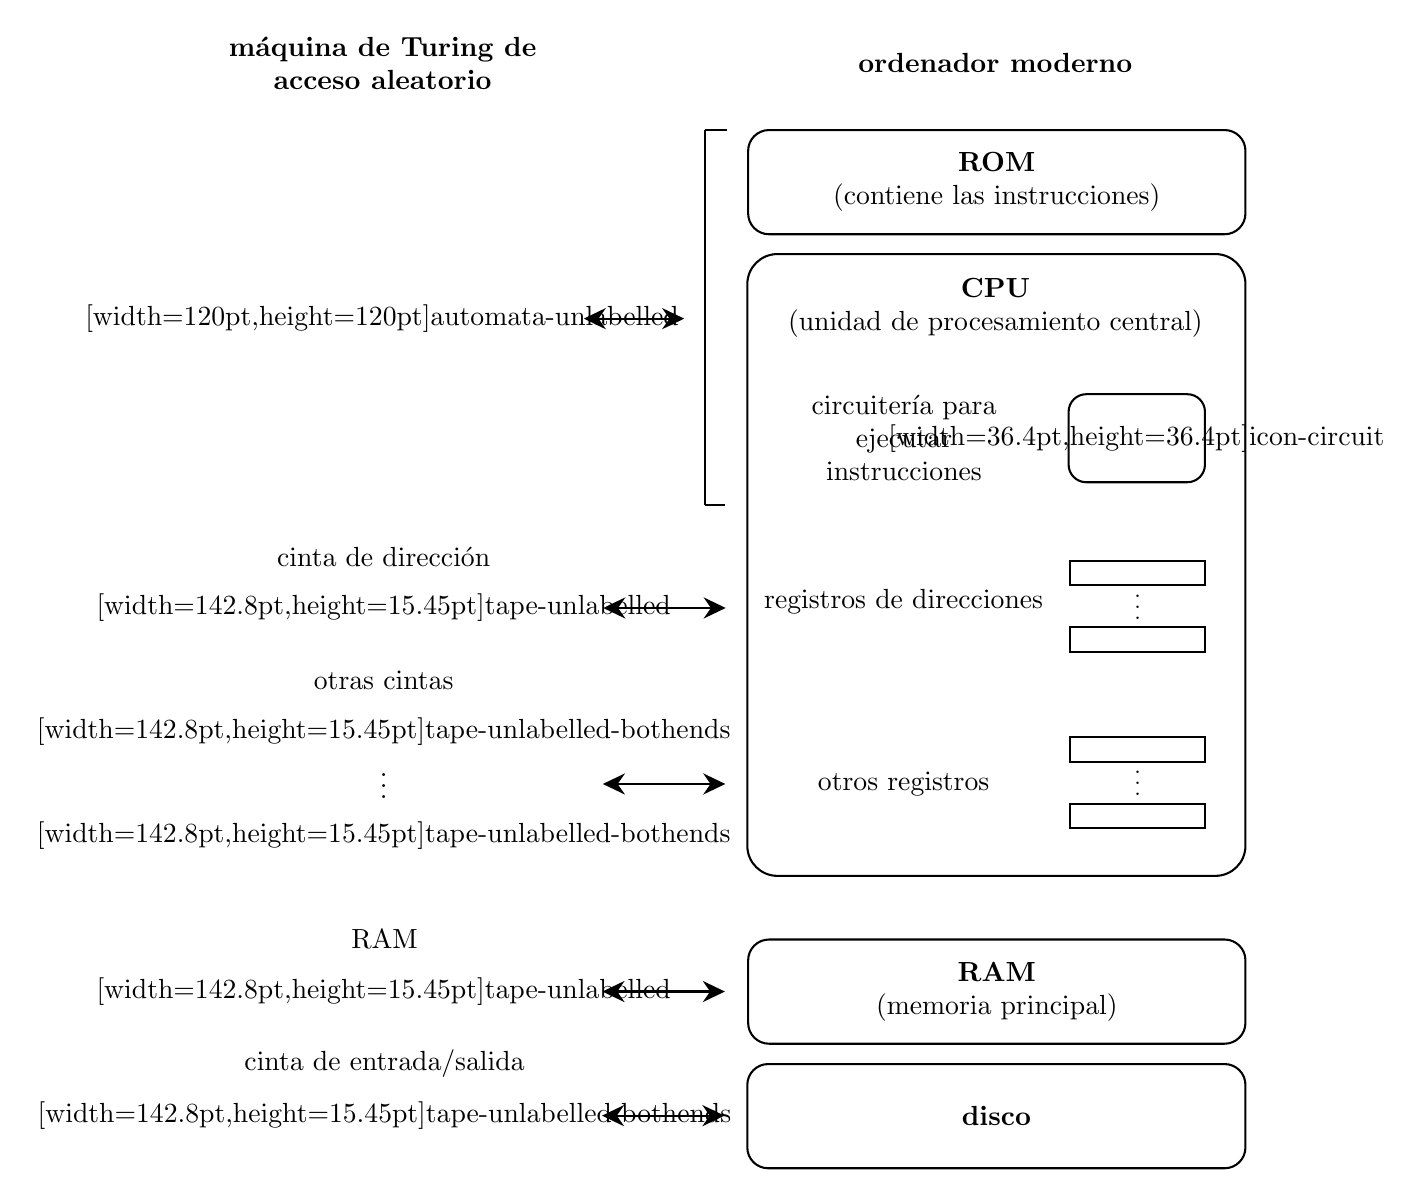
\begin{tikzpicture}[x=0.75pt,y=0.75pt,yscale=-1,xscale=1]
%uncomment if require: \path (0,629); %set diagram left start at 0, and has height of 629

%Image [id:dp5052356785139098] 
\draw (144,160.6) node  {\includesvg[width=120pt,height=120pt]{automata-unlabelled}};
%Rounded Rect [id:dp16008108582529212] 
\draw   (320.4,80.04) .. controls (320.4,74.5) and (324.9,70) .. (330.44,70) -- (549.96,70) .. controls (555.5,70) and (560,74.5) .. (560,80.04) -- (560,110.16) .. controls (560,115.7) and (555.5,120.2) .. (549.96,120.2) -- (330.44,120.2) .. controls (324.9,120.2) and (320.4,115.7) .. (320.4,110.16) -- cycle ;
%Rounded Rect [id:dp8550659349752405] 
\draw   (320,144.24) .. controls (320,136.24) and (326.49,129.75) .. (334.49,129.75) -- (545.51,129.75) .. controls (553.51,129.75) and (560,136.24) .. (560,144.24) -- (560,414.85) .. controls (560,422.85) and (553.51,429.33) .. (545.51,429.33) -- (334.49,429.33) .. controls (326.49,429.33) and (320,422.85) .. (320,414.85) -- cycle ;
%Rounded Rect [id:dp3980421004805672] 
\draw   (320.4,470.04) .. controls (320.4,464.5) and (324.9,460) .. (330.44,460) -- (549.96,460) .. controls (555.5,460) and (560,464.5) .. (560,470.04) -- (560,500.16) .. controls (560,505.7) and (555.5,510.2) .. (549.96,510.2) -- (330.44,510.2) .. controls (324.9,510.2) and (320.4,505.7) .. (320.4,500.16) -- cycle ;
%Rounded Rect [id:dp8207352186926025] 
\draw   (320,530.04) .. controls (320,524.5) and (324.5,520) .. (330.04,520) -- (549.96,520) .. controls (555.5,520) and (560,524.5) .. (560,530.04) -- (560,560.16) .. controls (560,565.7) and (555.5,570.2) .. (549.96,570.2) -- (330.04,570.2) .. controls (324.5,570.2) and (320,565.7) .. (320,560.16) -- cycle ;
%Image [id:dp4653438326616097] 
\draw (144.8,300.3) node  {\includesvg[width=142.8pt,height=15.45pt]{tape-unlabelled}};
%Shape: Rectangle [id:dp231624424338565] 
%\draw   (475.2,294.6) -- (540.2,294.6) -- (540.2,306.26) -- (475.2,306.26) -- cycle ;
%Shape: Rectangle [id:dp8216158761938366] 
\draw   (475.6,362.6) -- (540.6,362.6) -- (540.6,374.26) -- (475.6,374.26) -- cycle ;
%Straight Lines [id:da7645694678182564] 
\draw    (253.6,300.26) -- (306.6,300.26) ;
\draw [shift={(309.6,300.26)}, rotate = 180] [fill={rgb, 255:red, 0; green, 0; blue, 0 }  ][line width=0.08]  [draw opacity=0] (10.72,-5.15) -- (0,0) -- (10.72,5.15) -- (7.12,0) -- cycle    ;
\draw [shift={(250.6,300.26)}, rotate = 0] [fill={rgb, 255:red, 0; green, 0; blue, 0 }  ][line width=0.08]  [draw opacity=0] (10.72,-5.15) -- (0,0) -- (10.72,5.15) -- (7.12,0) -- cycle    ;
%Straight Lines [id:da441650131991439] 
\draw    (253.4,385.06) -- (306.4,385.06) ;
\draw [shift={(309.4,385.06)}, rotate = 180] [fill={rgb, 255:red, 0; green, 0; blue, 0 }  ][line width=0.08]  [draw opacity=0] (10.72,-5.15) -- (0,0) -- (10.72,5.15) -- (7.12,0) -- cycle    ;
\draw [shift={(250.4,385.06)}, rotate = 0] [fill={rgb, 255:red, 0; green, 0; blue, 0 }  ][line width=0.08]  [draw opacity=0] (10.72,-5.15) -- (0,0) -- (10.72,5.15) -- (7.12,0) -- cycle    ;
%Straight Lines [id:da026287841550500568] 
\draw    (253.2,485.06) -- (306.2,485.06) ;
\draw [shift={(309.2,485.06)}, rotate = 180] [fill={rgb, 255:red, 0; green, 0; blue, 0 }  ][line width=0.08]  [draw opacity=0] (10.72,-5.15) -- (0,0) -- (10.72,5.15) -- (7.12,0) -- cycle    ;
\draw [shift={(250.2,485.06)}, rotate = 0] [fill={rgb, 255:red, 0; green, 0; blue, 0 }  ][line width=0.08]  [draw opacity=0] (10.72,-5.15) -- (0,0) -- (10.72,5.15) -- (7.12,0) -- cycle    ;
%Straight Lines [id:da39421236199134] 
\draw    (253,544.86) -- (306,544.86) ;
\draw [shift={(309,544.86)}, rotate = 180] [fill={rgb, 255:red, 0; green, 0; blue, 0 }  ][line width=0.08]  [draw opacity=0] (10.72,-5.15) -- (0,0) -- (10.72,5.15) -- (7.12,0) -- cycle    ;
\draw [shift={(250,544.86)}, rotate = 0] [fill={rgb, 255:red, 0; green, 0; blue, 0 }  ][line width=0.08]  [draw opacity=0] (10.72,-5.15) -- (0,0) -- (10.72,5.15) -- (7.12,0) -- cycle    ;
%Straight Lines [id:da9170493361927601] 
\draw    (299.4,250.86) -- (309.4,250.86) ;
%Straight Lines [id:da15556503654230558] 
\draw    (299.4,69.86) -- (310.4,69.86) ;
%Straight Lines [id:da21370062507016763] 
\draw    (299.4,69.86) -- (299.4,250.86) ;
%Straight Lines [id:da659991079227169] 
\draw    (244.2,160.86) -- (286.6,160.86) ;
\draw [shift={(289.6,160.86)}, rotate = 180] [fill={rgb, 255:red, 0; green, 0; blue, 0 }  ][line width=0.08]  [draw opacity=0] (10.72,-5.15) -- (0,0) -- (10.72,5.15) -- (7.12,0) -- cycle    ;
\draw [shift={(241.2,160.86)}, rotate = 0] [fill={rgb, 255:red, 0; green, 0; blue, 0 }  ][line width=0.08]  [draw opacity=0] (10.72,-5.15) -- (0,0) -- (10.72,5.15) -- (7.12,0) -- cycle    ;
%Image [id:dp8580690474170394] 
\draw (507.49,218.48) node  {\includesvg[width=36.4pt,height=36.4pt]{icon-circuit}};
%Rounded Rect [id:dp036199891504040904] 
\draw   (474.8,205.75) .. controls (474.8,201.07) and (478.6,197.27) .. (483.28,197.27) -- (532.01,197.27) .. controls (536.69,197.27) and (540.49,201.07) .. (540.49,205.75) -- (540.49,231.2) .. controls (540.49,235.88) and (536.69,239.68) .. (532.01,239.68) -- (483.28,239.68) .. controls (478.6,239.68) and (474.8,235.88) .. (474.8,231.2) -- cycle ;
%Image [id:dp8048596501026082] 
\draw (144.8,359.9) node  {\includesvg[width=142.8pt,height=15.45pt]{tape-unlabelled-bothends}};
%Image [id:dp1557490659088474] 
\draw (144.8,484.9) node  {\includesvg[width=142.8pt,height=15.45pt]{tape-unlabelled}};
%Image [id:dp0736655278860916] 
\draw (145.2,544.7) node  {\includesvg[width=142.8pt,height=15.45pt]{tape-unlabelled-bothends}};
%Image [id:dp5610473288355018] 
\draw (144.8,409.9) node  {\includesvg[width=142.8pt,height=15.45pt]{tape-unlabelled-bothends}};
%Shape: Rectangle [id:dp7129304699861174] 
\draw   (475.6,394.6) -- (540.6,394.6) -- (540.6,406.26) -- (475.6,406.26) -- cycle ;


\draw   (475.6,277.6) -- (540.6,277.6) -- (540.6,289.26) -- (475.6,289.26) -- cycle ;
\draw   (475.6,309.6) -- (540.6,309.6) -- (540.6,321.26) -- (475.6,321.26) -- cycle ;

% Text Node
\draw (440.2,95.1) node   [align=left] {\begin{minipage}[lt]{162.7pt}\setlength\topsep{0pt}
\begin{center}
\textbf{ROM}\\(contiene las instrucciones)
\end{center}

\end{minipage}};
% Text Node
\draw (439.53,155.55) node   [align=left] {\begin{minipage}[lt]{162.7pt}\setlength\topsep{0pt}
\begin{center}
\textbf{CPU}\\(unidad de procesamiento central)
\end{center}

\end{minipage}};
% Text Node
\draw (395.5,218.33) node   [align=left] {\begin{minipage}[lt]{88.17pt}\setlength\topsep{0pt}
\begin{center}
circuitería para ejecutar instrucciones
\end{center}

\end{minipage}};
% Text Node
\draw (395.33,297.17) node   [align=left] {\begin{minipage}[lt]{102pt}\setlength\topsep{0pt}
\begin{center}
registros de direcciones
\end{center}

\end{minipage}};
% Text Node
\draw (395.33,385.17) node   [align=left] {\begin{minipage}[lt]{102pt}\setlength\topsep{0pt}
\begin{center}
otros registros
\end{center}

\end{minipage}};
% Text Node
\draw (440.2,485.1) node   [align=left] {\begin{minipage}[lt]{162.7pt}\setlength\topsep{0pt}
\begin{center}
\textbf{RAM}\\(memoria principal)
\end{center}

\end{minipage}};
% Text Node
\draw (440,545.1) node   [align=left] {\begin{minipage}[lt]{162.7pt}\setlength\topsep{0pt}
\begin{center}
\textbf{disco}
\end{center}

\end{minipage}};
% Text Node
\draw (439.5,37.75) node   [align=left] {\begin{minipage}[lt]{162.52pt}\setlength\topsep{0pt}
\begin{center}
\textbf{ordenador moderno}
\end{center}

\end{minipage}};
% Text Node
\draw (144.3,37.75) node   [align=left] {\begin{minipage}[lt]{128.79pt}\setlength\topsep{0pt}
\begin{center}
\textbf{máquina de Turing de}\\\textbf{acceso aleatorio}
\end{center}

\end{minipage}};
% Text Node
\draw (145.2,519.83) node   [align=left] {\begin{minipage}[lt]{129.47pt}\setlength\topsep{0pt}
\begin{center}
cinta de entrada/salida
\end{center}

\end{minipage}};
% Text Node
\draw (145.2,459.83) node   [align=left] {\begin{minipage}[lt]{129.47pt}\setlength\topsep{0pt}
\begin{center}
RAM
\end{center}

\end{minipage}};
% Text Node
\draw (144.8,275.43) node   [align=left] {\begin{minipage}[lt]{129.47pt}\setlength\topsep{0pt}
\begin{center}
cinta de dirección
\end{center}

\end{minipage}};
% Text Node
\draw (144.8,382.03) node   [align=left] {\begin{minipage}[lt]{129.47pt}\setlength\topsep{0pt}
\begin{center}
$\vdots$
\end{center}

\end{minipage}};
% Text Node
\draw (144.8,335.03) node   [align=left] {\begin{minipage}[lt]{129.47pt}\setlength\topsep{0pt}
\begin{center}
otras cintas
\end{center}

\end{minipage}};
% Text Node
\draw (508.1,380.76) node   [align=left] {\begin{minipage}[lt]{44.2pt}\setlength\topsep{0pt}
\begin{center}
{\footnotesize $\vdots$}
\end{center}

\end{minipage}};

\draw (508.1,295.76) node   [align=left] {\begin{minipage}[lt]{44.2pt}\setlength\topsep{0pt}
\begin{center}
{\footnotesize $\vdots$}
\end{center}

\end{minipage}};

\end{tikzpicture}
\caption{Simulación de un ordenador moderno a través de una máquina de Turing de acceso aleatorio}
\label{fig:simulacion-mtr-ordenador}
\end{figure}
% ===================+
\vfill
\pagebreak

% ===================+
\begin{proposicion}\label{prop:python-a-monocinta}
Una máquina de Turing de una sola cinta puede ser simulada por un programa en Python.
\end{proposicion}
\begin{proof}
Para probar esto, deberemos de crear un programa en Python que, dada la descripción de una máquina de Turing de una sola cinta $M=$, sea capaz de aplicar todos los pasos de cálculo y devolver la configuración en la que la máquina para.
\vspace{8pt}
% ====================
\begin{lstlisting}[language=Python, caption=\lstinline{simula_turing.py},label={lst:simula-turing}]
import utilidades
from turing import Turing|\label{line:simula-turing-turing}|

def simula_turing(entrada):|\label{line:simula-turing-main}|
    codificacion_maquina, entrada_maquina = utilidades.UAM(entrada)|\label{line:simula-turing-uam}|

    # creamos la máquina de Turing a partir de la entrada de la función SISO
    maquina_turing = Turing(codificacion_maquina, entrada_maquina)|\label{line:simula-turing-codificamaq}|

    # ejecutamos la máquina
    maquina_turing.ejecutar()|\label{line:simula-turing-ejecutar}|

    # si llegamos aquí, la máquina ha parado: devolvemos su configuración
    return str(maquina_turing)|\label{line:simula-turing-return}|
\end{lstlisting}
% ====================

Podemos ver la simulación en el \cref{lst:simula-turing}. Hay más información sobre dónde encontrar y cómo usar el código de este trabajo en el \cref{ap:codigo-trabajo}. Explicaremos cada una de las líneas.

En primer lugar, en la \cref{line:simula-turing-turing}, se importa la clase \lstinline{Turing} del paquete \lstinline{turing}. Puedes encontrar el código de \texttt{turing.py} en la carpeta \texttt{codigo}. Esta clase se encarga de instanciar una máquina de Turing, e incorpora las funciones necesarias para realizar la simulación.

En la \cref{line:simula-turing-main} tenemos nuestra función \emph{main}, que acepta un \emph{string} como entrada. Para poder codificar varias entradas, recurrimos a las funciones \texttt{MAU} y \texttt{UAM} de la librería \texttt{utilidades}. Dado una lista de \emph{strings}, la función \texttt{MAU} (de \emph{Múltiple A Uno}) los convierte en un único \emph{string} usando la cadena \palabra{::} como separador. La función \texttt{UAM} realiza el proceso contrario, y convierte un \emph{string} en una lista de \emph{strings}, separando por la cadena \palabra{::}.

De este modo, el \emph{string} de entrada tendrá la forma
$$
    \texttt{CODIFICACIÓN} + \texttt{\textquotesingle::\textquotesingle} + \texttt{ENTRADA}
$$
Es decir, estará compuesto de los \emph{strings} correspondientes a la codificación de la máquina de Turing y a la entrada unidos por \palabra{::}.

Codificar una máquina de Turing\index{codificación!de una máquina de Turing} $M$ mediante un \emph{string} es sencillo. Lo haremos mediante archivos, que no son más que cadenas de caracteres. Codificaremos cada uno de los estados y símbolos con \emph{strings}, y crearemos una cadena de caracteres uniendo las siguientes cadenas de caracteres mediante saltos de línea, en este orden:
\begin{itemize}
    \item Los estados, separados por espacios.
    \item Los símbolos del alfabeto de entrada, separados por espacios.
    \item Los símbolos del alfabeto de trabajo, separados por espacios.
    \item El símbolo blanco.
    \item El estado inicial.
    \item Los estados finales, separados por espacios.
    \item Una línea para cada transición
        $$\delta(\texttt{EA}, \texttt{SL})=(\texttt{ES}, \texttt{SR}, \texttt{M})$$
    (donde \texttt{EA} es el estado actual, \texttt{SL} es el símbolo leído, \texttt{ES} es el estado siguiente, \texttt{SR} es el símbolo de reemplazo y \texttt{M} es el movimiento, pudiendo \texttt{M} ser \texttt{I}, \texttt{D} o \texttt{S}), con el siguiente formato:
    $$
        \texttt{EA, SL : ES, SR, M}
    $$
\end{itemize}

En la \cref{line:simula-turing-uam}, separamos la entrada y guardamos la codificación de la máquina en \linebreak\texttt{codificacion\_maquina} y la entrada en \texttt{entrada\_maquina}, mediante la función \texttt{UAM} anteriormente explicada.

En la \cref{line:simula-turing-codificamaq}, creamos una instancia de la clase \texttt{Turing} con la codificación de la máquina y la entrada. Al crear la instancia, se ejecutarán funciones que comprueban si la descripción es correcta. En caso de haber un error, la máquina no ejecutará ningún paso y la salida de la \cref{line:simula-turing-return} será de tipo error.

En la \cref{line:simula-turing-ejecutar}, ejecutamos la máquina, aplicando transición tras transición hasta que pare. En caso de no parar, el programa en Python tampoco parará.

En la \cref{line:simula-turing-return}, devolvemos la configuración de la máquina al haber parado, y si acepta o rechaza.

De esta forma hemos simulado $M$ mediante un programa en Python.
\end{proof}
% ===================+

El programa \texttt{simula\_turing} está implementado y se encuentra disponible en el repositorio de este trabajo (véase el \cref{ap:codigo-trabajo}). Mostraremos un ejemplo de la codificación explicada, y cómo usarlo, mediante el \cref{ej:simula-turing}.

\begin{ejemplo}\label{ej:simula-turing}
Una codificación de la máquina $M_{\#a>\#b}$ del \cref{ej:mt-1} puede ser:\footnote{Incluimos comentarios y líneas vacías, que ignoraremos}

\begin{lstlisting}[language=Python]
q_0 q_a q_b q_R q_F     # estados
a b                     # alfabeto de entrada
a b X _                 # alfabeto de trabajo
_                       # símbolo blanco
q_0                     # estado inicial
q_F                     # estados finales

# transiciones
q_0, a : q_a, X, D
q_0, b : q_b, X, D
q_0, X : q_0, X, D
q_a, a : q_a, a, D
q_a, b : q_R, X, I
q_a, X : q_a, X, D
q_a, _ : q_F, _, S
q_b, a : q_R, X, I
q_b, b : q_b, b, D
q_b, X : q_b, X, D
q_R, a : q_R, a, I
q_R, b : q_R, b, I
q_R, X : q_R, X, I
q_R, _ : q_0, _, D
\end{lstlisting}

Esta codificación se encuentra en el archivo \texttt{codigo/maquinas\_turing/mas\_a\_que\_b.mt}. Para probar \texttt{simula\_turing.py}, basta abrir el intérprete de Python en la carpeta \texttt{codigo} y ejecuta las siguientes sentencias:

\begin{lstlisting}[numbers=none,frame=none]
>>> from utilidades import leer, MAU
>>> from simula_turing import simula_turing
>>> codificacion = leer('./maquinas_turing/mas_a_que_b.mt')
>>> entrada = 'aababb'
\end{lstlisting}
En este caso hemos puesto $aababb$ como entrada, pero puedes reemplazarla por cualquier entrada de $\{a,b\}^*$. Para ejecutar la función \texttt{simular}, simplemente ejecuta:

\begin{lstlisting}[numbers=none,frame=none]
>>> simula_turing(MAU(codificacion, entrada))
'q_0 : X X X X X X [_] (rechaza)'
\end{lstlisting}
Vemos que el programa Python devuelve la cadena de caracteres $$\texttt{\textquotesingle{}q\_0 : X X X X X X [\_] (rechaza)\textquotesingle}$$Es decir, la máquina de Turing $M_{\#a>\#b}$ para en el estado
$$
    q_0\;:\;X\:X\:X\:X\:X\:X\:\fbox{\Vtextvisiblespace}
$$
que no es un estado final ($q_0 \notin F$), y por tanto la entrada $aababb$ es rechazada.
\end{ejemplo}

Puedes probar con cualquier entrada y con otras máquinas de Turing de la carpeta \linebreak\texttt{codigo/maquinas\_turing}. Algunos de los archivos corresponden a codificaciones incorrectas, para que puedas ver cómo \texttt{simula\_turing.py} es un programa en Python tal y como lo hemos definido (SISO, sin errores, etc.).

Una vez hemos probado la secuencia de simulaciones de la \cref{fig:cadena-simulaciones}, el teorema siguiente queda demostrado.

% ===================+
\begin{teorema}[Equivalencia entre programas en Python y máquinas de Turing]\label{teo:equivalencia}
Dado un programa en Python $P$, existe una máquina de Turing (de una sola cinta) $M$ que computa la misma función que $P$.
\end{teorema}
% ===================+

Acabamos de probar que las máquinas de Turing y los programas en Python son iguales en términos de los programas que podemos escribir en ellos. Esto nos será útil cuando definamos el concepto de \emph{problema} en el \cref{ch:problema-parada}.

\section{Relación con la tesis de Church-Turing}\label{sec:church-turing}\index{tesis de Church-Turing}

El trabajo que hemos realizado en este capítulo ha sido arduo, pero el resultado que hemos obtenido es extremadamente interesante. Sin embargo, debemos recordar que la elección del lenguaje de programación Python ha sido completamente arbitraria: podríamos sustituir a Python por cualquier otro lenguaje de programación capaz de codificar una máquina de Turing.

¿Qué nos dice esto de lo que puede ser computado? Podemos verlo de dos formas: por una parte, los programas en Python (así como los ordenadores en sí) no son más que máquinas de Turing con ``muchos atajos'' y extensiones. Por otra (y de forma más interesante), la máquina de Turing, que inicialmente puede parecer inocente por la sencillez de su descripción, tiene un potencial de cálculo enorme, pues puede ejecutar cualquier programa de ordenador.

En el \cref{ch:historia} ya expusimos la \emph{tesis de Church-Turing}. Por conveniencia, la referenciamos de nuevo a continuación.

\begin{adjustwidth}{30pt}{}
    \textbf{Tesis de Church-Turing.} \emph{Toda función calculable (algoritmo) puede calcularse mediante una máquina de Turing}
\end{adjustwidth}

Como hemos dicho, se trata de una tesis, es decir, es una afirmación que se supone pero que no se demuestra. Probar este resultado es prácticamente imposible, pero hay evidencias que lo refuerzan, como lo que acabamos de hacer: hemos visto cómo un modelo de computación, en apariencia, mucho más complejo que la máquina de Turing, resulta ser equivalente a ella.

Sin embargo, siempre existe la posibilidad de que avances en la comprensión de cómo se comporta el universo nos abran las puertas a nuevos y más potentes modelos de cálculo. Este no es el caso de la computación cuántica, que puede acelerar la resolución de algunos problemas, pero no amplía la gama de funciones calculables. \cite{Kaye2007}

Esta tesis tiene profundas implicaciones. Concluiremos este capítulo con algunas preguntas.

\begin{enumerate}
    \item ¿Es la mente humana una máquina de Turing?
    \item ¿Es el universo una máquina de Turing? Esto es, ¿son las leyes que rigen el universo (las leyes de la física) computables?
    \item En caso de que esto no sea así, ¿es posible crear una máquina más poderosa que la de Turing?
\end{enumerate}

Respecto a la primera pregunta, es importante realizar una puntualización histórica: Turing afirmaba que la respuesta era afirmativa, es decirm que la mente humana podría simularse en un ordenador. Esta tesis fue central en sus trabajos de Inteligencia Artificial \cite{Turing1950}, en los que defendía que el desarrollo de esta disciplina solo era cuestión de tiempo.
%De este modo, podemos entender que este capítulo puede servir, de forma secundaria, como un

%: poder definir programas en este modelo es complejo y tedioso. Comprobaremos a partir de un sencillo ejemplo (\cref{ej:mt-1})

%En este capítulo la definiremos con precisión y profundizaremos, a través de modelos equivalentes, que la capacidad de computación

%Una de las tesis más fundamentales de las ciencias de la computación es la \emph{tesis de Church-Turing}, que es la noción intuitiva de que todo algoritmo o procedimiento es equivalente a una máquina de Turing.

%Nombrada por su inventor, Alan Turing, la máquina de Turing es un modelo matemático sencillo que pretende representar la noción de qué puede ser computado. En este capítulo, la definiremos con precisión y veremos, a través de modelos equivalentes, que la capacidad de computació

%Esta afirmación nos conduce directamente al corazón de los fundamentos teóricos de la computación, inicialmente expresada por Alonzo Church en el 1936

%Una de las herramientas más usadas actualmente en las ciencias de la computación son las máquinas de Turing, pues permiten describir de forma matemática y sencilla el concepto de \emph{computar}. Estas máquinas permiten demostrar múltiples resultados.

%En este capítulo, seguiremos el orden inverso al histórico, y no es por casualidad: tal y como comentamos en el \cref{ch:historia}


\endinput
